%\usepackage[spanish]{babel}
\chapter{Introducción}
Resultado de la masificación de uso de TIC en la industria, existe gran demanda por especialistas preparados en el área de las ciencias de la computación. En el estudio de esta materia, el aprendizaje de la programación, es uno de los temas más difíciles de aprender. En la resolución de problemas se requiere de elevadas habilidades analíticas y la aplicacion de conceptos abstractos. Por lo que estudiar estas ideas, es a menudo, un desafío \cite{improve}. En el ámbito del desarrollo de software, adjunto a las destrezas en programación, son necesarias el uso de metodologías, enfoques y herramientas que ayuden a ordenar el proceso de elaboración del software, con el fin de asegurar la producción de aplicaciones y sistemas de calidad, en donde las operaciones participantes de los procesos computarizados sean usables, confiables y mantenibles. 
Algunas universidades, en respuesta al actual funcionamiento de la industria, han implementado infraestructuras mas realistas para apoyar a los alumnos en su desarrollo \cite{Factory}, en el contexto del trabajo colaborativo, apoyado con herramientas estándar \cite{TOOL}  en conjunto con estrategias integradoras, diseñadas con el propósito de mejorar el desempeño académico, que luego se traduzca en graduados habilidosos, seguros y competentes.\\
A continuación, se ilustra una breve descripción de los capítulos y sus contenidos, donde se pueden apreciar las etapas de desarrollo de este trabajo.
El Capítulo 2 se definen los principales conceptos que seran abordados durante el desarrollo del trabajo.
Luego en el Capitulo 3 se definen el problema específico detectado y la solución propuesta. En la etapa de análisis, se especifican la definición de requerimientos, las funcionalidades que debe poseer la infraestructura. En el Capitulo de Diseño, se define se dividen las tareas y se definen las el modelo que se implementara.
En el Capítulo 8 se presenta la implementación de cada uno de los niveles que forman parte de sistema. Posteriormente, en el Capítulo 10, se realizan las pruebas correspondientes, que nos permitan asegurar con un grado aceptable de confianza y evidencia documentada, el funcionamiento correcto y constante del sistema, en condiciones normales y limites de operación. 
El capitulo 11 detalla los pasos que se llevaron a cabo para la implantación del sistema en su ambiente de producción. Finalmente, en el Capítulo 11, se exponen las conclusiones de este trabajo de título.

\chapter{Marco conceptual}

En este capítulo se definen los conceptos que formarán parte del dominio de la solución propuesta.\\

\section{Ingeniería de software}

Las ciencias de la computación e informática es un área compleja \cite{improve} que requiere entendimiento de las matemáticas, fundamentos de la computación y la aplicación de metodologías en el desarrollo de soluciones innovadoras. La enseñanza de esta práctica a tomado diferentes acercamientos durante el tiempo, dependiendo de cuales métodos se adapten mejor a un ambiente académico y/o a las necesidades de un determinado entorno. \\

El desempeño académico de los alumnos, normalmente, es medido por medio de pruebas, exámenes, quizzes, trabajos, etc. La principal misión en cada semestre, en gran parte de las instituciones que imparten carreras relacionadas a las ciencias de la computación e informática, es ofrecer educación de calidad en orden de producir hábiles y competentes graduados.\\

Aprender técnicas y lenguajes de programación es uno de los requerimientos para obtener el título de Ingeniero Civil en Informática en la Universidad de Valparaíso. Esta habilidad requiere el desarrollo del pensamiento creativo, que será de utilidad, en la construcción de software más complejo, donde es necesaria la aplicación de conceptos relacionados a la ingeniería de software para ordenar las ideas de los alumnos y optimizar la aplicación de las habilidades y competencias que progresivamente adquieren.\\


Las prácticas actuales en la enseñanza de Ingeniería de software no están preparando adecuadamente a los estudiantes para el mundo real \cite{resumen}. Se resume el problema en los siguientes puntos.\\

\begin{itemize}
	\item No hay producto: Los alumnos desarrollan proyectos en lugar de productos.
	\item Baja duración: Un semestre o dos, no hay continuidad.
	\item Alto recambio: Los alumnos no se están desarrollando en base a experiencias.
	\item Baja complejidad: Debido al tiempo que requiere entrenar las habilidades.
	\item No hay cliente: La mayoría de los proyectos no tiene contacto con un cliente.
\end{itemize}

Existe mucha literatura sobre acercamientos en la enseñanza de la Ingeniería de software, por muchos años fue enseñado el modelo en cascada, ya que era considerado la mejor estructura para el desarrollo de software, luego fue el modelo incremental \cite{Clinton}. Más recientes se tiene la programación extrema y los métodos ágiles \cite{agil}.


\section{Método ágil}

Los métodos de desarrollo ágil están intentado ofrecer respuestas a las organizaciones que buscan ciclos cortos de desarrollo con rápido proceso de elaboración del producto \cite{agilCloud}.
Los métodos ágiles se centran en resolver requerimientos  a través de procesos colaborativos de diseño, donde el software es continuamente liberado para que los desarrolladores y el usuario final puedan experimentar con las funcionalidades que se implementan a lo largo de este ciclo. 
Los desarrolladores implementan requerimientos de usuario en periodos cortos y los usuarios pueden revisar las funcionalidades creadas, para así dar su opinión y sugerencias (Feedback). Luego, los desarrolladores pueden tomar en cuenta estas opiniones y sugerencias en un ciclo futuro del desarrollo. Esto genera un ambiente altamente interactivo entre el desarrollador y el usuario del sistema, en consecuencia se tiene un rápido cumplimiento de los requerimientos de usuario. Estos métodos tienden a separar los requerimientos de un proyecto en segmentos más pequeños. Asegurando retroalimentación constante con el usuario en cada tarea e iteración del proyecto. Los segmentos son planeados, implementados y testeados individualmente, para mantener altos estándares de calidad.\\

\section{Nube de computo}

Puede ser definido como el uso de hardware computacional nuevo o existente y tecnologías de virtualización para formar una estructura compartida que proporciona servicios basados en la web. La 'Nube de computo' ofrece muchos beneficios a las organizaciones. Posibilita la colaboración entre comunidades y grupos de trabajo dispares, ha superado las dificultades que han afectado a soluciones comerciales existentes y facilitado el acceso a gran cantidad de recursos computacionales de forma eficiente. Los tres modelos predominantes son software, plataforma e Infraestructura como servicio. \\

\subsection{Virtualización}

La virtualización ya existe en el ecosistema de las tecnologías de la información y comunicación. Este concepto esconde complejidad subyacente que permite a múltiples clientes, con diversas aplicaciones y demandas, utilizar servidores de forma simultánea.\\


Los tres modelos dominantes son presentados en la [Figura 2.1]. En la capa superior, se encuentra el software como servicio (SaaS). En la segunda capa, se tiene Plataforma como servicio (PaaS). Por ultimo Infraestructure como servicio (IaaS).\\

\begin{figure}[H]
	\centering
	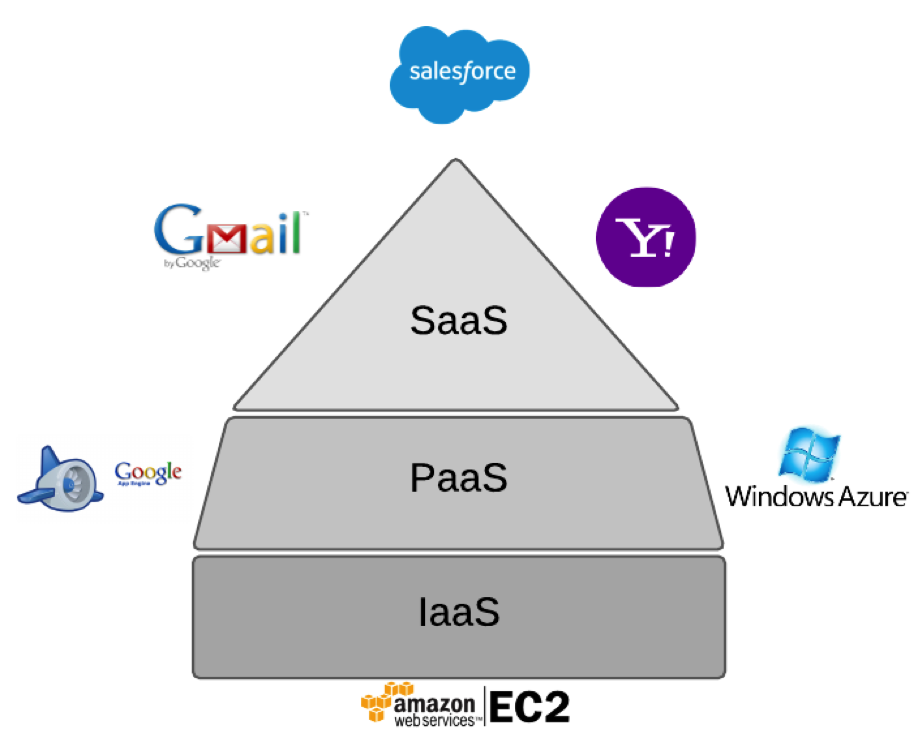
\includegraphics[width=0.4\linewidth]{img/MarcoTeorico}
	\caption{Virtualización en tres niveles}
	\label{fig:MarcoTeorico}
\end{figure}

\begin{itemize}
	\item Software como servicio: Permite a usuarios acceder a software y servicios que residen en la 'Nube' y no en el dispositivo de usuario. Los consumidores de aplicaciones 'SaaS' solo requieren de un pequeño cliente para hacer uso de estos recursos. Esto reduce los requerimientos de hardware para los usuarios finales. Algunos ejemplos populares son Gmail y Google Apps.\\
	
	\item Plataforma como servicio: Provee acceso a API’s, lenguajes de programación y capas intermedias, que permite a los suscriptores desarrollar aplicaciones personalizadas sin necesidad de instalar o configurar el entorno de desarrollo. Usando las herramientas incluidas en esta plataforma, desarrolladores pueden construir aplicaciones y servicios tomando ventaja del hardware virtualizado, redundancia de datos y alta disponibilidad. 
	Una vez el desarrollo es completado, la aplicación puede ser distribuida a los usuarios vía internet. Google App Engine, Microsoft Azure and SalesForce.com son ejemplos de PaaS.\\
	
	\item Infraestructura como servicio: Puede ser definido como el uso de servidores, almacenamiento y virtualización para facilitar servicios a los usuarios. La infraestructura consiste en las instalaciones, redes de comunicación, nodos físicos de computo y lote de recursos computacionales virtualizados y administrados por los proveedores de servicios.\\
	
\end{itemize}


\section{Control de versiones}

Se denomina versión, al estado en el que se encuentra un producto en el tiempo. El control de versiones tiene que ver con la gestión de los cambios generados en los elementos que componen un producto. Si bien, este control puede ser realizado manualmente [Figura 2.2].

\begin{figure}[H]
	\centering
	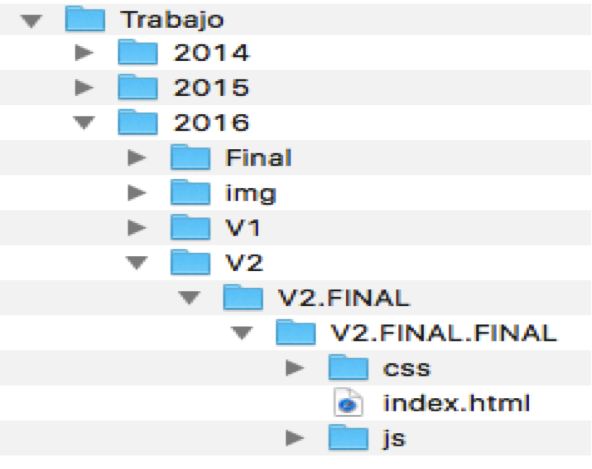
\includegraphics[width=0.4\linewidth]{img/VersionManual}
	\caption{Sistema manual de control de versiones}
	\label{fig:MarcoTeorico}
\end{figure}

En la industria informática son utilizados los sistemas de control de versiones [SCV] para la gestion del código fuente de proyectos. Estas herramientas facilitan principalmente el almacenamiento de archivos, la recuperación de cada uno de ellos y el registro histórico e identificación de las modificaciones realizadas en las sucesivas versiones.
En general, es beneficioso el uso de SCV debido a su capacidad de potencia el trabajo en paralelo y distribuido, facilitando la realización de cambios y respectiva unión entre ellos.
Cuando un elemento es bloqueado, impidiendo que otros usuarios puedan hacer uso de éste, nos encontramos bajo un esquema de funcionamiento exclusivo.
Por otro lado, si grupos de usuarios pueden trabajar sobre un mismo elemento, estamos en presencia de un esquema colaborativo.

\subsection{Esquemas de almacenamiento}

\begin{itemize}
	\item Centralizados: Estos sistemas, como CVS, Subversion, y Perforce, tienen un único servidor que contiene todos los archivos versionados, y varios clientes que descargan las versiones desde ese repositorio central. La edición de un archivo especifico no soporta multiples usuarios y se requiere estar conectados constantemente al repositorio central [Figura 2.3].
	
	\begin{figure}[H]
		\centering
		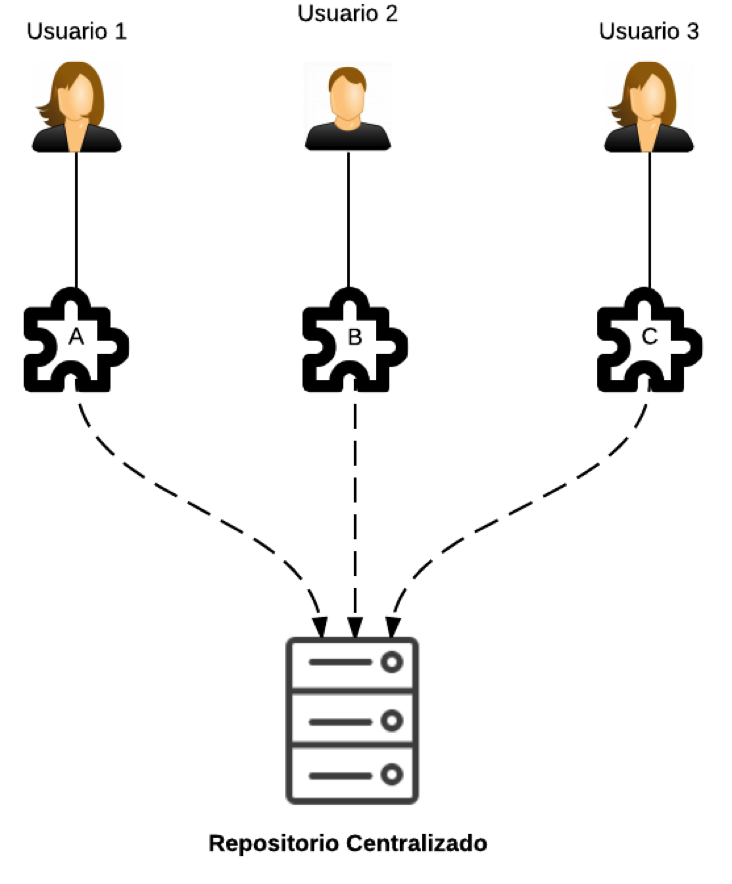
\includegraphics[width=0.3\linewidth]{img/Centralizado}
		\caption{Esquema simplificado de un sistema de control de versiones centralizado}
		\label{fig:MarcoTeorico}
	\end{figure}
\end{itemize}

\subsubsection{Principales características de los sistemas centralizados}

\begin{enumerate}
	\item Control central del avance del proyecto.
	\item La mayoría de las operaciones requieren conexión con el repositorio central.
	\item Una versión contiene la copia del directorio completo.
\end{enumerate}

\begin{itemize}
	\item Distribuidos: Este sistema descentralizado [Figura 2.4] permite que muchos desarrolladores trabajen sobre un mismo proyecto, sin necesidad de requerir una red común. Cada usuario tiene una copia local de toda la información de un repositorio, la cual puede modificar cualquier archivo y sincronizar los aportes cuando desee, haciendo uso de una conexión a internet.
\end{itemize}

\begin{figure}[H]
	\centering
	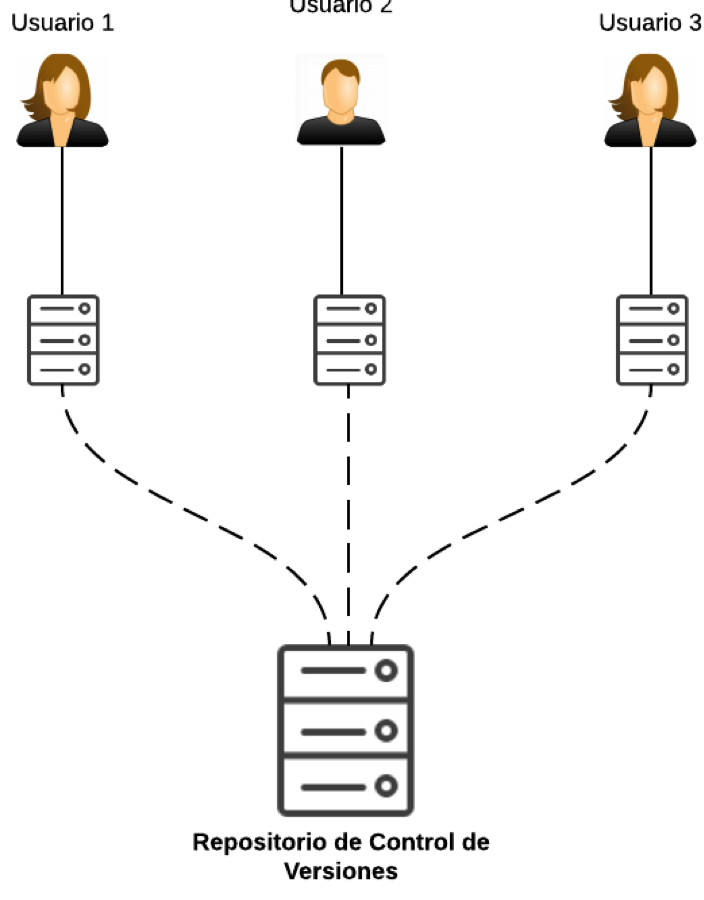
\includegraphics[width=0.3\linewidth]{img/Distribuido}
	\caption{Esquema simplificado de un sistema de control de versiones distribuido}
	\label{fig:MarcoTeorico}
\end{figure}

\subsubsection{Principales características de los sistemas distribuidos}

\begin{enumerate}
	\item Cada desarrollador tiene su propia copia local.
	\item Capacidad de regresar a una versión anterior de manera local.
	\item Los repositorios distribuidos funcionan como respaldo.
	\item Es posible realizar cambios sobre cualquier archivo del repositorio.
	\item Unión de los cambios.
\end{enumerate}

\section{Marco Técnologico}

\chapter{Estado del arte}

\section{Sistemas, técnicas y/o métodos actuales}

La industria se queja que los actuales planes de estudios de las universidades fallan en cuestiones prácticas del desarrollo real de software, muchas empresas esperan que los graduados en ciencias de la computación sean productivos, sin necesidad de entrenamiento adicional \cite{a1,a2,a3}. Los alumnos no están siendo preparados para enfrentar el desarrollo a gran escala, donde es requerido el trabajo en equipo, habilidades de comunicación oral/escrita entre otras competencias.

Para enfrentar esta situación las infraestructuras colaborativas son utilizadas en la enseñanza de diferentes aspectos del desarrollo de software. En \cite{AR} el análisis de requerimientos se practica haciendo uso de equipos y entornos colaborativos. Varias universidades han creado entornos más realistas para la enseñanza de aspectos del desarrollo colaborativo de software \cite{Factory} en \cite{TOOL} se analizan las herramientas y sus perspectivas de uso.
La naturaleza colaborativa y los principios claves del código libre son discutidos en \cite{OS}. También algunas Universidades han enseñado la Ingeniería de software usando ambientes de aprendizaje \cite{Oss} para ayudar a los alumnos en temas básicos y avanzados de las ciencias de la computación. En \cite{Long} son usadas herramientas de código libre con el fin de brindar experiencias más realistas a los alumnos.
Existen comunidades tales como Teaching Open Source \cite{Open}, dedidacado a promover la investigación y los métodos colaborativos.

 “The software Factory”: este concepto es aplicado por algunas Universidades, que a través de infraestructura y herramientas de trabajo colaborativo, proponen a sus alumnos interactuar con su entorno, solucionando problemas reales de la industria, bajo la guía de la facultad \cite{Factory}.The Catholic University of America (CUA) es una pequeña institución en el corazón de Washington D.C. que utiliza el concepto de ‘software factory’ para enseñar a sus alumnos a desarrollar software. El proceso se modelaa en la [Figura 3.1].A cada nivel, rol y responsabilidad le corresponde un color.

\begin{figure}[H]
	\centering
	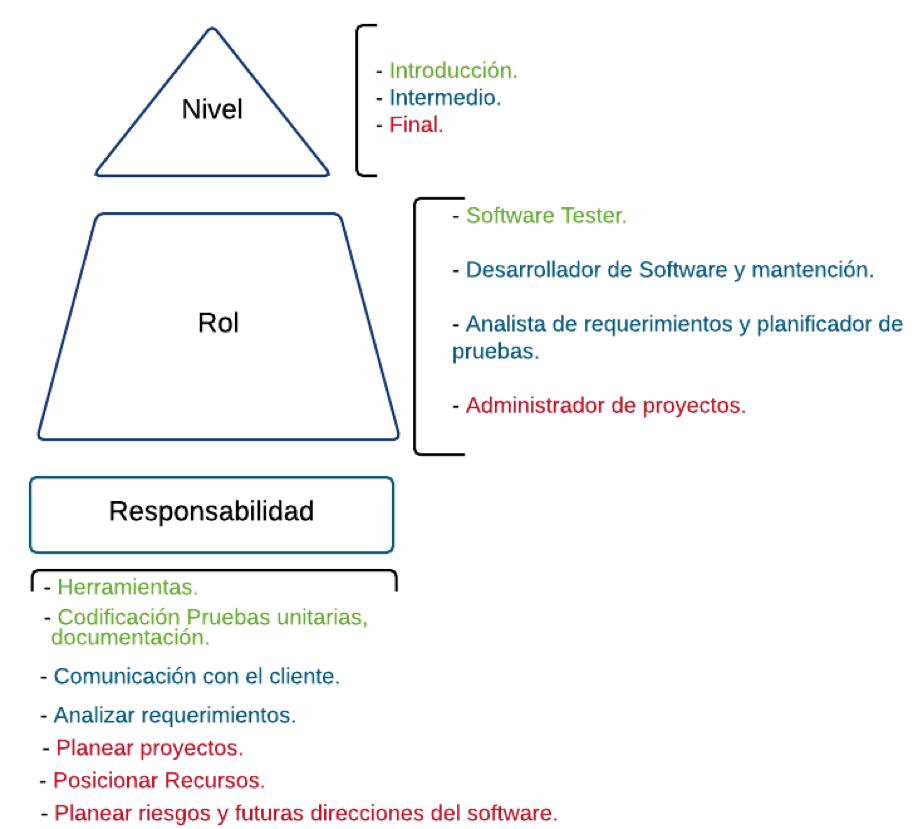
\includegraphics[width=8.5cm]{img/arte}
	\caption {Abstracción del plan de estudio de la Universidad}
	\label{fig:dcu}
\end{figure}


\begin{itemize}
	\item Semestre 1 - Desarrollo de software y herramientas: En esta primera etapa se introduce a los alumnos al desarrollo de software y al conjunto de herramientas disponibles. 
	\item Semestre 2 - Software System Testing: En este curso los alumnos son puestos en el rol de Software testers, con todas las responsabilidades que esto implica.
	\item Semestre 3 - Desarrollo de Software y Mantención: En este curso los alumnos son puestos en el rol de desarrolladores con responsabilidades tales como escribir Software, realizar pruebas unitarias, documentar, etc.
	\item Semestre 4 - Desarrollo de Software y mantención: Este curso es la continuación de S3.
	\item Semestre 5 - Requerimientos y plan de pruebas: En este nivel los alumnos son puestos en el rol de analistas de requerimientos de sistema y test planners. Algunas de las responsabilidades aquí son: Comunicarse con el cliente, analizar los requerimientos del cliente, documentación, etc.
	\item Semestre 6 - Software Tesing: En este nivel los alumnos son puestos en el rol de diseñador de software.
	\item Semestre 7 - Administración de proyectos: En este curso los alumnos son puestos en el rol de administradores de proyectos. Las responsabilidades del alumno incluyen: Planear proyectos, posicionar recursos, estimar riesgos y planear futuras direcciones del software. 
\end{itemize} 	

	\subsubsection{Análisis crítico}
	
	Con el uso explosivo uso de la internet y la permeabilidad de la tecnología en prácticamente cada aspecto de nuestras vidas, la necesidad de personal capacitado para construir software de calidad es aparente. La industria desea que las instituciones educacionales prepararen a los estudiantes en el uso de las últimas tecnologías. Pero las Universidades hacen énfasis en desarrollar habilidades de largo plazo. Ya que enfocarse en satisfacer las demandas de la industria significaría comprometer la calidad de los conocimientos del alumno. El enfoque pedagógico de las Universidades evita que al volverse obsoletas las tecnologías, ocurra lo mismo con los conocimientos del estudiante. El problema de esto, son los aspectos prácticos del desarrollo de software, usualmente no se transfiere la suficiente experiencia, que permita apreciar las implicancias de las decisiones que toman los alumnos durante el ciclo de vida del software.	

\chapter{Definición del problema y solución propuesta}

\section{Contexto}

Producto del rápido avance tecnológico en la industria, existe una gran demanda por especialistas preparados en el área de las ciencias de la computación. En el estudio de esta materia, el aprendizaje de la programación incluye el uso de lenguajes y sintaxis que permiten la implementación de modelos abstractos codificados (datos, control). Por lo que aprender y estudiar estas ideas, es a menudo, un desafío. Los procesos asociados al desarrollo de sistemas son una tarea compuesta de aspectos teóricos y cognitivos, en donde son necesarias tanto habilidades en programación como la aplicación de enfoques sistemáticos que guíen el desarrollo software, con el fin de asegurar que las operaciones participantes de los procesos computarizados sean usables, confiables y mantenibles.
El perfil de egreso de la carrera de Ingeniería Civil en Informática de la Universidad de Valparaíso caracteriza a los futuros profesionales como Integradores de las tecnologías [9]. El desarrollo de estas competencias se adquiere conforme el alumno avanza por las etapas que componen el plan de estudio.
En una primera fase, el alumno resuelve tareas especificas mediante secuencias de instrucciones o algoritmos. En una etapa intermedia, asocia y comunica estos programas con el fin de ejecutar un conjunto de coordinadas funciones, tareas o actividades que satisfagan requerimientos de pequeños proyectos. Finalmente el alumno es capas de ejectar actividades de planificación, control y gestión de proyectos.\\
Los Alumnos  aplican el aprendizaje acomodando los conceptos a un modelo que basa sus operaciones en un ambiente local. Este posee las herramientas suficientes para el desarrollo de cada una de las prácticas que requieran de estructura computacional para llevar a cabo sus funciones [Figura 4.1].

\begin{figure}[H]
	\centering
	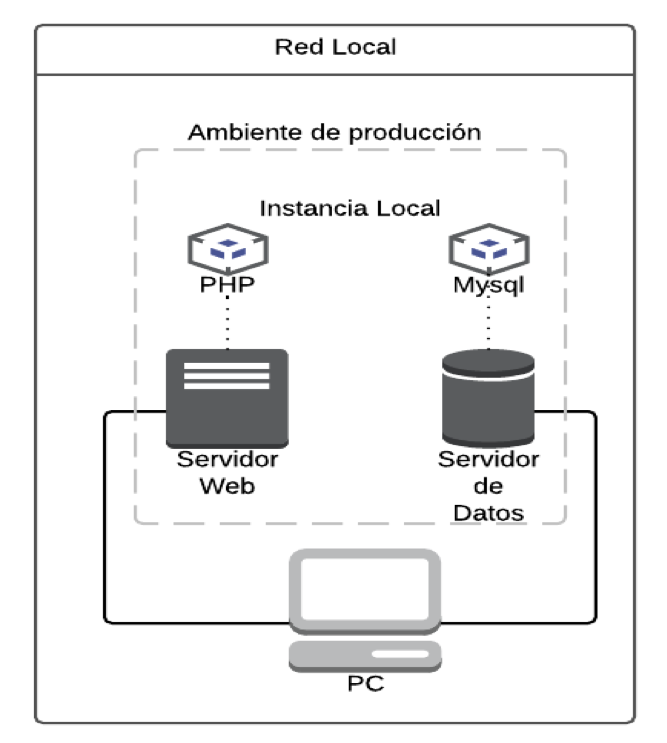
\includegraphics[width=0.3\linewidth]{img/Situacionactual}
	\caption{Modelo de la situación actual}
	\label{fig:MarcoTeorico}
\end{figure}


Consecuencia de este esquema, el desarrollo de las actividades, es reducido al trabajo individual o de pequeños grupos, con la difícil tarea de coordinar aportes y gestionar los cambios cuando el equipo crece o se dispersa. 
Por otro lado, este modelo no representa adecuadamente la realidad del desarrollo de software, que existe hoy, en las organizaciones, donde los futuros Ingenieros deberán ser capaces de Integrar tecnologías en un contexto dinámico, hoy en día los productos son altamente susceptibles al cambio y es común tener a múltiples desarrolladores, en diferentes labores, accediendo concurrentemente a un mismo proyecto.
Dado este escenario, es de vital importancia que los alumnos puedan aplicar los contenidos de las asignaturas usando herramientas y ambientes similares a las organizaciones, con el fin de otorgar experiencias que eventualmente puedan transferir a situaciones reales.\\ 

\section{Solución propuesta}

Implementación de una infraestructura [Figura 4.2]. Que proporcione recursos para el uso de tecnologías y metodologías de apoyo a los alumnos en la aplicación de las materias. Haciendo uso de herramientas estándar que faciliten la enseñanza-aprendizaje. Construyendo en el alumno, desde una etapa temprana de su formación, una visión de las actividades asociadas al ciclo de vida del software.

\begin{figure}[H]
	\centering
	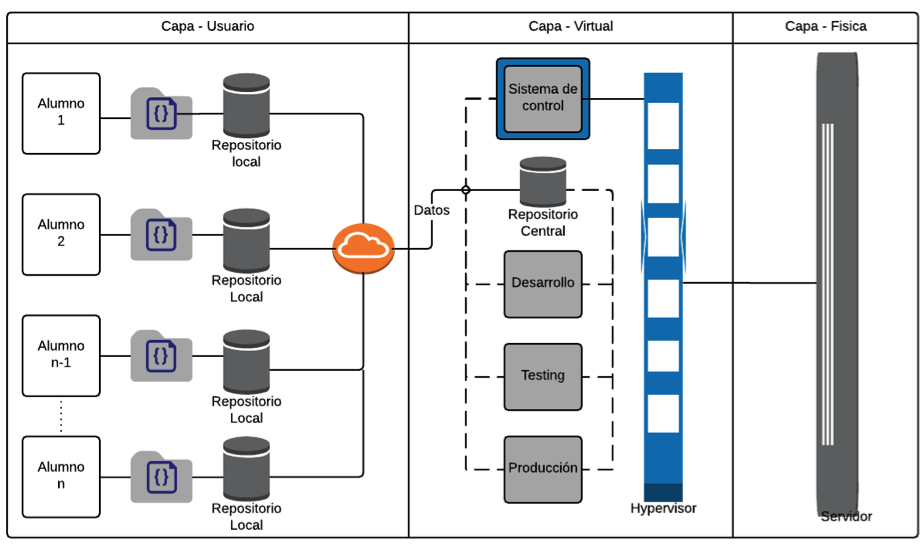
\includegraphics[width=0.25\linewidth]{img/Solucion}
	\caption{Arquitectura de alto nivel de la solución}
	\label{fig:MarcoTeorico}
\end{figure}

\section{Naturaleza del cambio}

Actualmente la Escuela de Ingeniería Civil en Informática no posee una plataforma que fomente el trabajo en equipo en ambientes similares a los que existen en la industria, donde los flujos de trabajo, uso de las tecnologías y recursos, están definidos y estructurados acorde a metodologías modernas
\cite{agilCloud}.

\section{Objetivos}

En esta sección se da a conocer el objetivo general del trabajo de título, junto con los objetivos específicos que permiten alcanzarlo.

\subsection{Objetivo general}

\begin{itemize}
	\item Implementar una infraestructura que permita el uso de herramientas que apoyen el desarrollo de software colaborativo en la Carrera de Ingeniería Civil en Informática de la Universidad de Valparaíso, con fines docentes, para integración de prácticas entre asignaturas.
\end{itemize}

\subsection{Objetivos específicos}

\begin{itemize}
	\item Especificar requerimientos y requisitos del sistema.
	\item Definir características del hardware disponible.
	\item Diseñar  modelo de la solución.
	\item Definir Tecnologías adecuadas para el diseño de la infraestructura.
	\item Realizar diagramado acorde a la etapa de desarrollo e implementación del sistema. 
	\item Definir políticas y flujos de trabajo.
	\item Determinar el funcionamiento constante y correcto de las funcionalidades del sistema.
\end{itemize}

\section{Aporte}
Como consecuencia de la implementación de este sistema. Se dispondrá de una Herramienta para conformar ambientes (redes, servidores, otros servicios) en donde alumnos, haciendo uso de tecnologías concretas, almacenen, administren y/o compartan distintas versiones de uno o varios proyectos haciendo uso de avances y recursos tecnológicos que hoy tienen raíces en la red.
\section{Metodología de investigación y desarrollo}

\subsection{Investigación}

Para la búsqueda de conceptos, tecnologías, trabajos y/o Investigaciones relacionadas a este tema, fueron utilizaron bibliotecas digitales [IEEE, ACM] en donde es posible descargar documentos haciendo uso de la red de la Universidad de Valparaíso.

\subsection{Desarrollo}


Metodología cascada, integrando el principio de trabajo en cadena, de manera de obtener resultados continuos en base a cada incremento [Figura 4.3].

\begin{figure}[H]
	\centering
	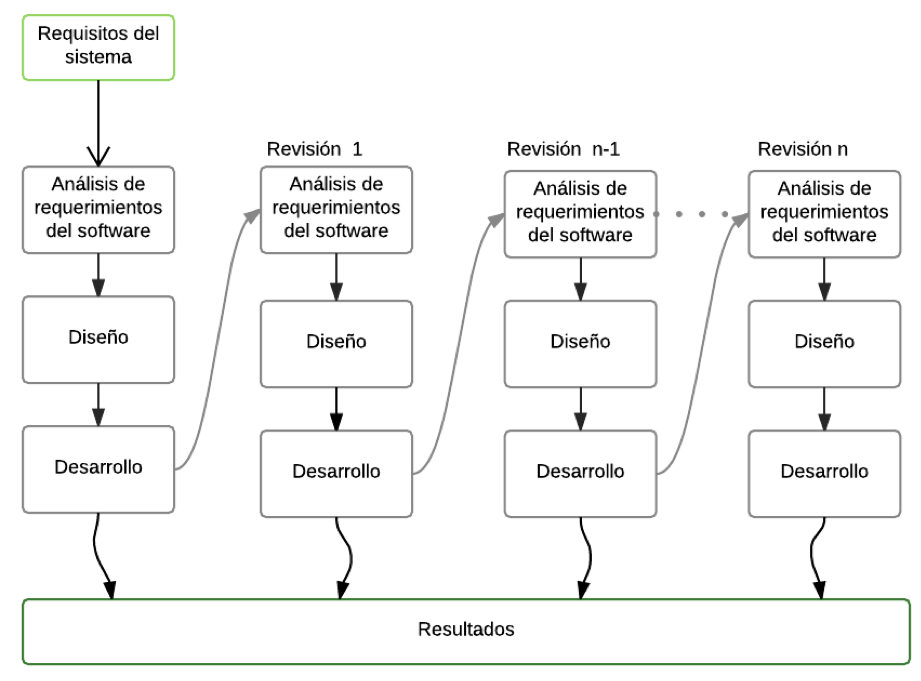
\includegraphics[width=0.33\linewidth]{img/Metodologia}
	\caption{Metodología de trabajo}
	\label{fig:MarcoTeorico}
\end{figure}

\chapter{Análisis}\label{sec:analisis}

En el siguiente capítulo se presenta el análisis realizado a través de investigaciones y reuniones en conjunto con el profesor guía del presente trabajo de título. 

\section{Especificación de requerimientos}

\subsection{Requerimientos funcionales}

\begin{itemize}
	\item RF1: Servidor dedicado al ramo de programación en lenguaje C.
	\item RF2: El servidor en C debe tener los programas Make, gcc y vim instalados.
	\item RF3: Creación y configuración de la integración continua, en un servidor dedicado, haciendo uso del la herramienta Jenkins.
	\item RF4: Estructura operacional para programación en lenguaje Java.
	\item RF5: Estructura operacional para programación en lenguaje .NET.
	\item RF6: Estructura operacional para programación en lenguaje PHP.
	\item RF7: Acceso a un sistema de control de versiones.
	\item RF8: Servidores para el despliegue del software.
\end{itemize}      
\subsection{Requerimientos no funcionales}
\begin{itemize}
	\item RNF: El servidor debe estar disponible el 95 porciento del tiempo (Alta disponibilidad).
\end{itemize}


\section{Diagrama de casos de uso (DCU)}

El diagrama de casos de uso representa las operaciones que los usuarios realizan en el sistema, junto con las relaciones existentes entre cada una de las tareas [Figura 5.1]. \\

\begin{figure}[H]
	\centering
	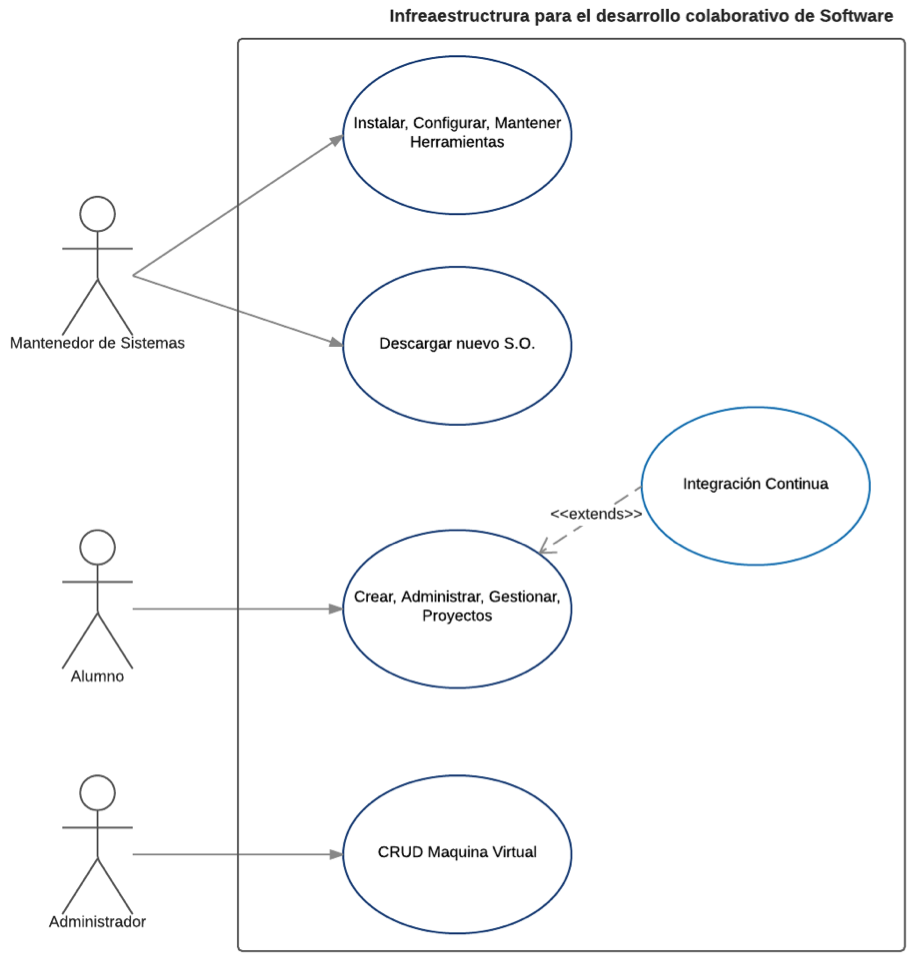
\includegraphics[width=7cm]{img/DCU}
	\caption {Diagrama de casos de uso}
	\label{fig:dcu}
\end{figure}

\chapter{Diseño}

En este Capítulo se presentan los niveles que comprenden el sistema a implementar:

\begin{itemize}
	\item Nivel Físico.
	\item Nivel Virtual.
	\item Nivel Conceptual.
	\item Herramientas.
\end{itemize}

\section{Diseño arquitectónico}

La solución tecnológica presentada en la [Figura 6.1] posee un nivel físico, que corresponde, a los recursos base de esta implementación. El nivel virtual brinda una mapeo dinámico del nivel Físico haciendo uso de un hipervisor. El nivel conceptual correspode a la metodologia que ordena el proceso de desarrollo de software, en este caso, se trata de un enfoque ágil. Finalmente se encuentra el conjunto de herramientas para facilitar el desarrollo colaborativo de software.
A continuación en la [Figura 6.2] se presenta la solución general, donde los usuarios a través de herramientas podrán resolver actividades académicas en ambientes colaborativos:

\begin{figure}[H]
	\centering
	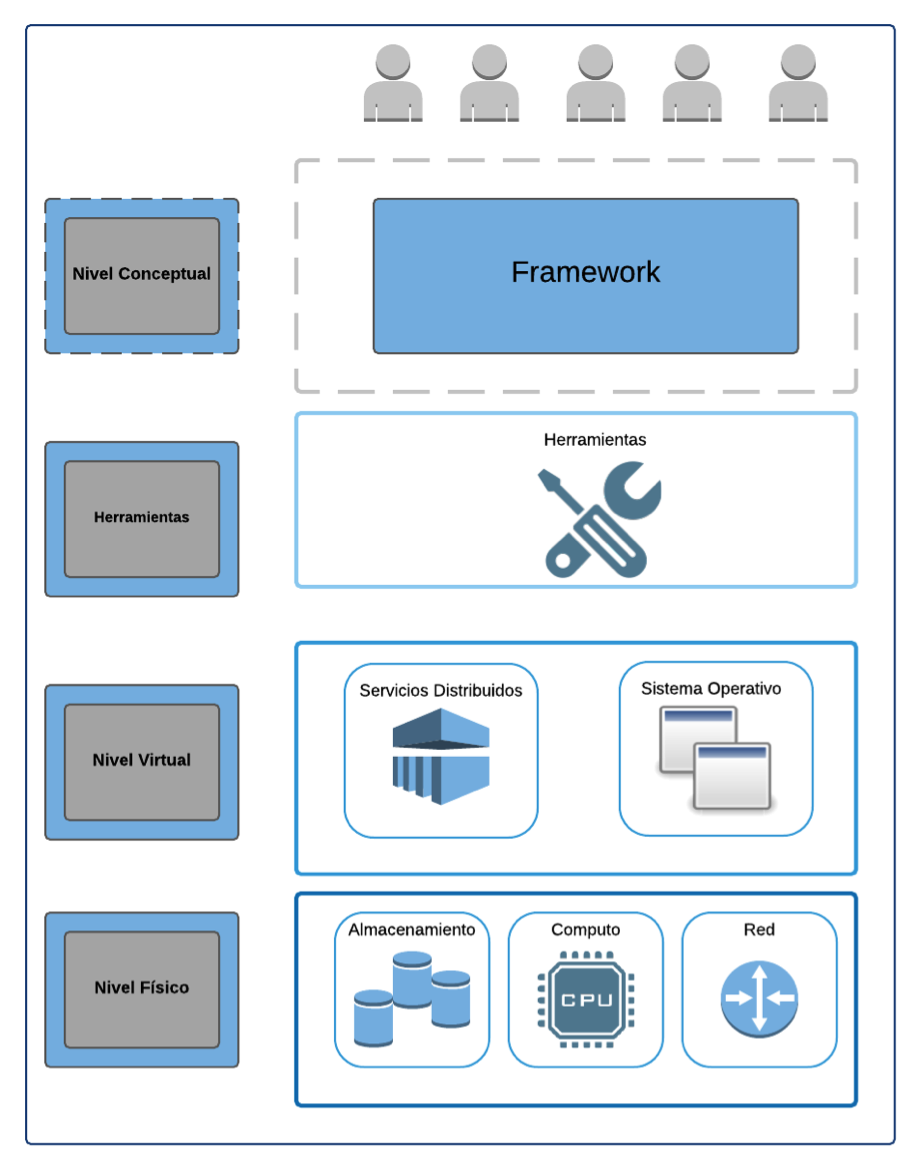
\includegraphics[width=6cm]{img/altonivel2}
	\caption {Diagrama general de la solución}
	\label{fig:dcu}
	
\end{figure}

\section{Descomposición arquitectural}

\subsection{Nivel Físico}
Este nivel encapsula el lote de recursos físicos disponibles para ser administrados y reorganizados según las necesidades que se presenten [Figura 6.3]. 

\begin{itemize}
	\item CPU.
	\item Almacenamiento.
	\item Red.
\end{itemize}


\begin{figure}[H]
	\centering
	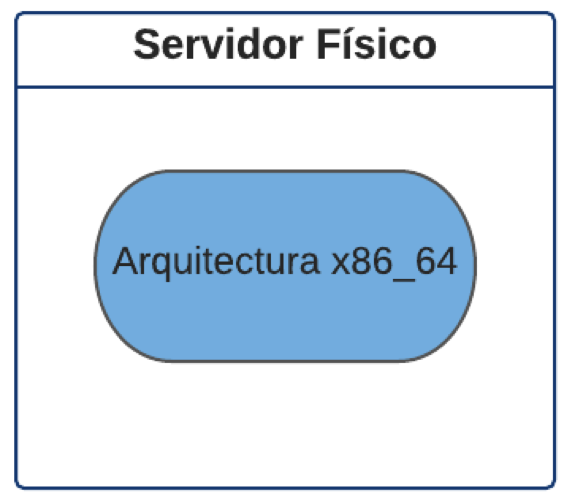
\includegraphics[width=3cm]{img/fisico}
	\caption {Nivel Físico}
	\label{fig:dcu}
\end{figure}

\subsection{Nivel virtual}

La implementación de esta capa tiene como finalidad particionar los recursos físicos, para ejecutar múltiples instancias de servidores. 
Los dos acercamientos típicamente utilizados son la arquitectura Hypervisor y Hosted. 
La arquitectura Hosted ofrece servicios de particionamiento un nivel por encima del sistema operativo estándar de esa maquina. Esto quiere decir,  existe un bloque adicional entre el metal y la virtualización [Figura 6.4].
Por otro lado, la implementación B  elimina este nivel, por medio de la instalación de un sistema operativo especial o hipervisor. La relación de adyacencia proporciona un acceso a los recursos de hardware más eficiente con el fin de ofrecer mayor robustez, escalabilidad y desempeño de las maquinas virtuales.

\begin{figure}[H]
	\centering
	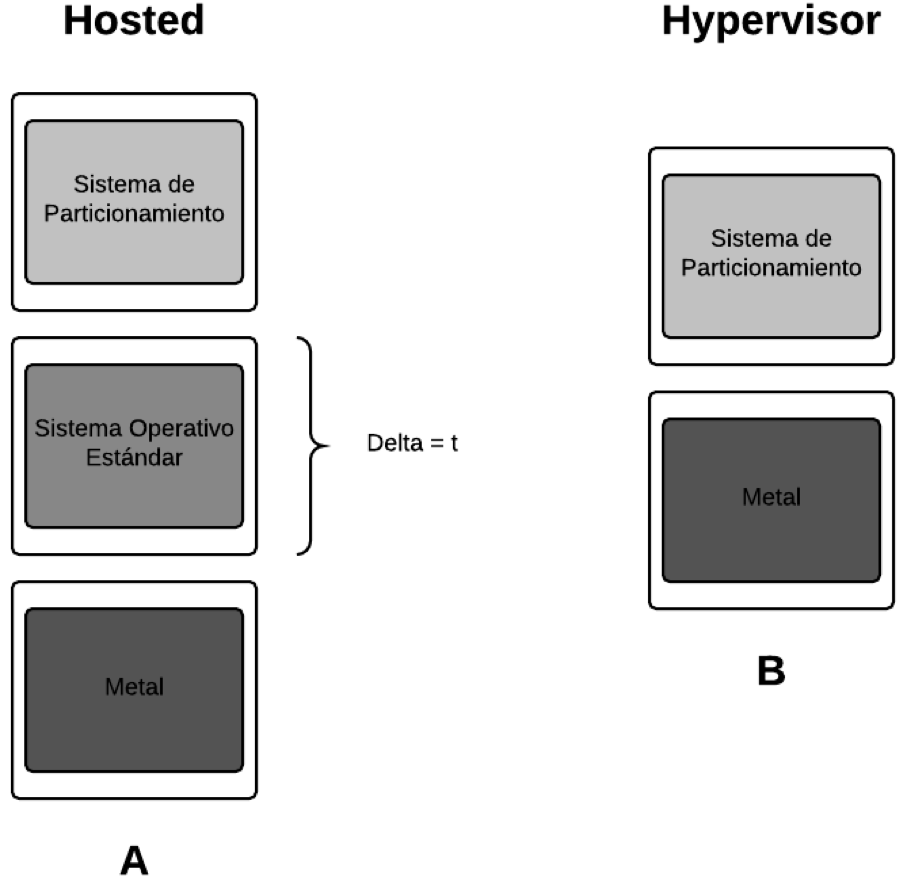
\includegraphics[width=6cm]{img/virtual}
	\caption {Arquitectura hosted v/s hypervisor}
	\label{fig:dcu}
\end{figure}

La figura 6.5 que se presenta a continuación ofrece mayor detalle del sistema de particionamiento a usar.

\begin{figure}[H]
	\centering
	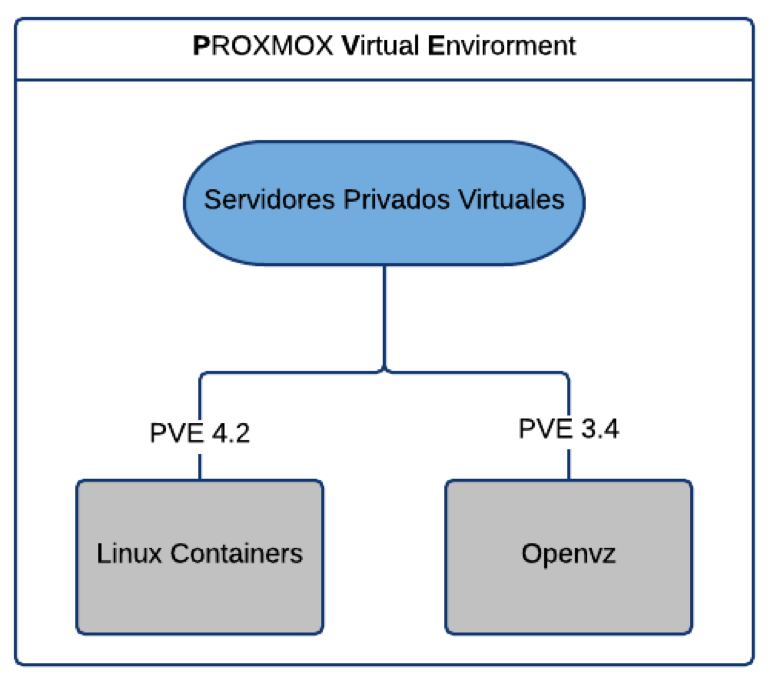
\includegraphics[width=4cm]{img/virtual2}
	\caption {Esquema del nivel virtual}
	\label{fig:dcu}
\end{figure}

Proxmox VE esta basado en debían (GNU/Linux).
Este sistema ofrece dos tipos de solución para la virtualización a nivel de sistema operativo. La tecnologia de virtualizacion cambia dependiendo de la version de Proxmox.

\subsubsection{Open Virtuozzo (OpenVZ)}

Es una tecnología de virtualización a nivel de sistema operativo para Linux. Permite a un servidor físico ejecutar múltiples instancias de servidores. El nucleo OpenVZ provee aislamiento, administración de recursos y toleracia a fallos. OpenVZ se encuentra disponible en la versión 3.4 del sistema pperativo Proxmox Virtual Envirorment.

\subsubsection{Container-Based Virtualization (LXC)}

Similar a la tecnología de virtualización OpenVZ, Linux-VServer y de otros sistemas pperativos como FreeBSD jail y Solaris Containers. Linux Containers permite la priorización de recursos (CPU, Memoria, Entrada/Salida, Red, Etc) sin necesidad de iniciar la maquina virtual. Esta herramienta combina Kernel cgroups para namespace aislados que proveen ambientes aislados y limpios para la ejecutar aplicaciones. LXC se encuentra disponible en la versión 4.2 del sistema operativo Proxmox.

\section{Nivel conceptual}

El objetivo principal de las metodologías ágiles es producir y entregar software funcional de forma rapida.
FDD es uno de los seis acercamientos que fueron presentados con el nacimiento del manifesto ágil, este fue creado por 17 individuos en 2001.
FDD es un modelo iterativo-incremental que consiste en la aplicación de cinco etapas [Figura 6.6]. Las ultimas dos etapas son repetidas hasta que el producto es completado, luego, el proyecto es formalmente cerrado. Este Framework descompone las actividades asociadas al desarrollo de un sistema en partes pequeñas que puedan ser resueltas en no mas de dos semanas. Estas piezas son llamadas ‘Características’, las cuales son tangibles, verificables por el usuario, aportan valor al cliente por si solas y tienen un tiempo de desarrollo que no excede las dos semanas. Las tareas son realizadas por los integrantes del proyecto, estos desempeñan distintos roles dentro de la organización, jerarquizados, que a su vez le corresponden una conjunto de responsabilidades [Figura 6.12].

\begin{figure}[H]
	\centering
	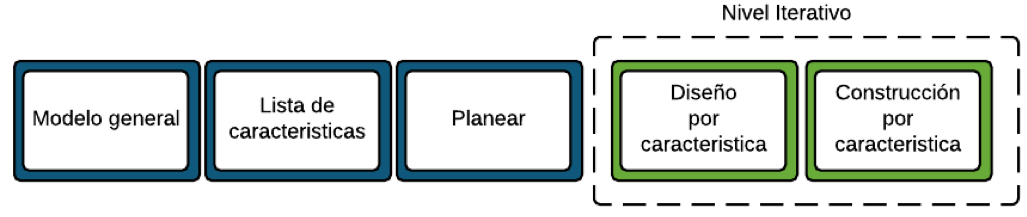
\includegraphics[width=10cm]{img/flow}
	\caption {Diagrama de bloques del proceso}
	\label{fig:dcu}
\end{figure}


\subsection{Modelo general}

Los expertos en el dominio realizan un recorrido de alto nivel del alcance del sistema y su contexto.

\subsubsection{Criterio de inicio de esta etapa}

Ya fueron seleccionados los expertos de dominio, programador jefe  y arquitecto adecuados para este proyecto.

\subsubsection{Tareas de esta etapa}

\begin{itemize}
	\item Formar un equipo para el modelado.
	\item Estudio de documentación asociada al dominio.
	\item Entregar información general del área de dominio a modelar.
	\item Formar grupos de modelado mas pequeños.
\end{itemize}

\subsubsection{Criterio para el cierre de esta etapa}

El equipo de modelado debe producir un modelo en conformidad con el arquitecto jefe del proyecto.

\subsubsection{Salidas}

\begin{itemize}
	\item Diagramas de clases.
	\item Diagrama de secuencia, si corresponde.
\end{itemize}

\subsubsection{Diagarama de flujo de trabajo} 

\begin{figure}[H]
	\centering
	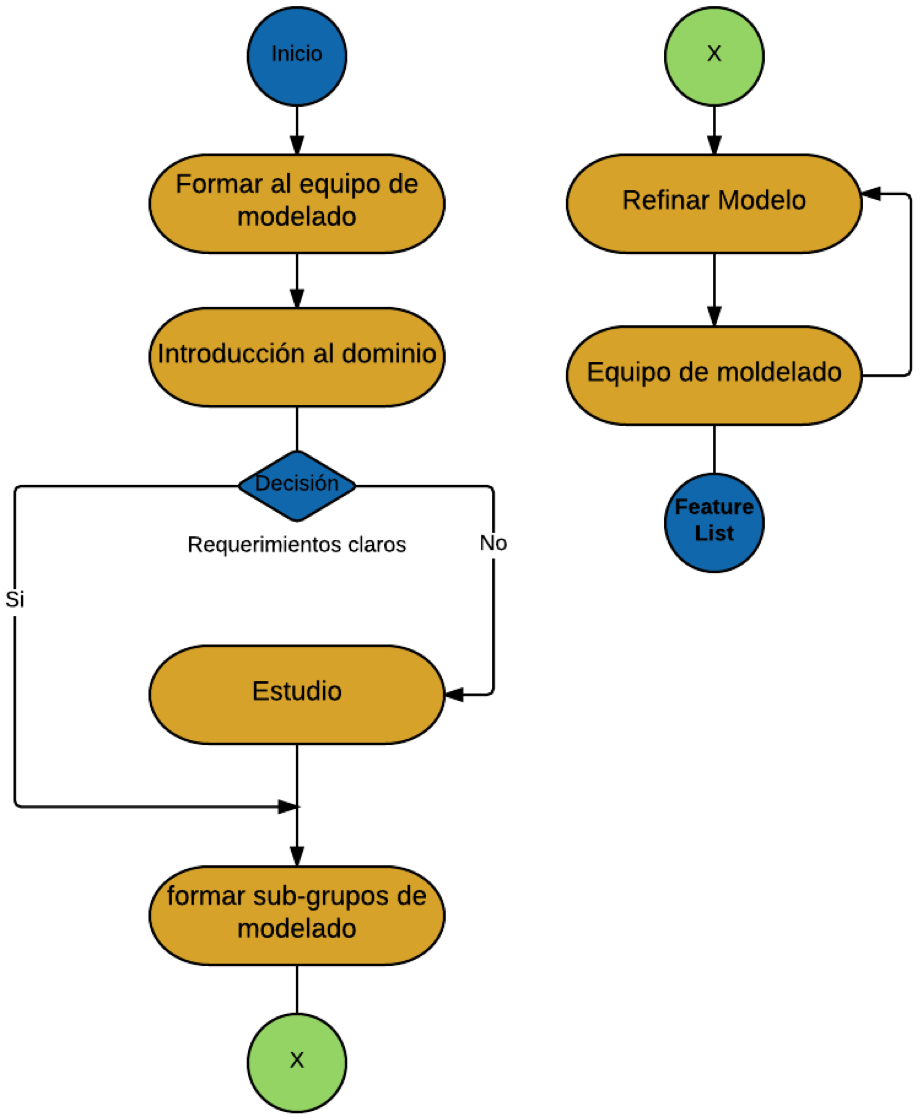
\includegraphics[width=3cm]{img/flujo1}
	\caption {Diagrama de flujo de la primera etapa.}
	\label{fig:dcu}
\end{figure}

\subsection{Lista de características}

El producto a desarrollar es descompuesto en una lista de actividades, esta lista corresponde a pequeñas piezas que aportan valor al cliente y  son expresadas de la forma Acción-Resultado-Objeto.
Las funcionalidades que son parte del dominio son descompuestas y distribuidas en las diferentes áreas. 
Por lo que cada área posee un numero acotado de ‘Características’. Como resultado, se tiene un listado jerarquizado de funcionalidades.

\subsubsection{Criterio para el inicio de esta etapa}

\begin{itemize}
	\item El equipo de modelamiento a completado exitosamente su trabajo.
\end{itemize}
\subsubsection{Tareas para esta etapa}
\begin{itemize}
	\item Formar el equipo para este proceso.
	\item Construir la lista de características.
\end{itemize}

\subsubsection{Roles participantes de esta etapa.}

Administrador de proyecto, administrador de desarrollo.

\subsubsection{Criterio para el cierre de esta etapa}

Como salida se debe tener una lista de características aprobada por administrador de proyecto y desarrollo.

\subsubsection{Salida}
\begin{itemize}
	\item Lista general de características por área.
\end{itemize}

\subsubsection{Diagarama de flujo de trabajo}
\begin{figure}[H]
	\centering
	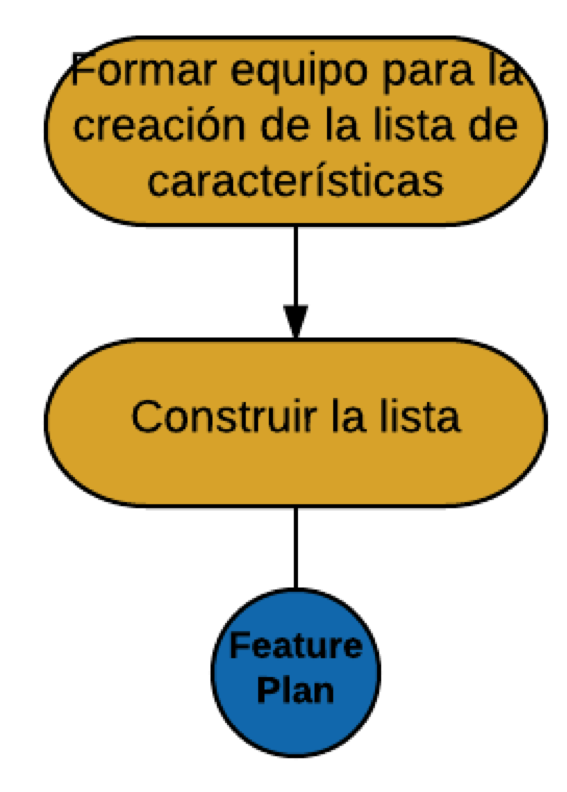
\includegraphics[width=2cm]{img/flujo2}
	\caption {Diagrama de flujo de la segunda etapa.}
	\label{fig:dcu}
\end{figure}

\subsection{Planear por característica}

En esta etapa se planea el orden en que serán implementadas las características. Para esto nos basamos en las dependencias, complejidad e importancia de cada una dentro del sistema a construir.\\

\subsubsection{Criterio para el inicio de esta etapa}
\begin{itemize}
	\item  La lista de características a sido completada con éxito.
\end{itemize}

\subsubsection{Tareas de esta etapa}
\begin{itemize}
	\item Formar el equipo para este proceso.
	\item Determinar la secuencia de desarrollo.
	\item Asignar un grupo de características al Programador Jefe.
	\item Asignar clases a los desarrolladores.
\end{itemize}
\subsubsection{Roles participantes de esta etapa}
Administrador de proyecto, Administrador de desarrollo, Programador jefe.
\subsubsection{Criterio para el cierre de esta etapa}
El proceso es cerrado en conformidad con el administrador de proyecto y desarrollo.

\subsubsection{Salida}
\begin{itemize}
	\item Lista de características con sus respectivas fechas.
	\item Programador jefe asignado a la lista de características.
	\item Lista de clases para los programadores.
\end{itemize}

\subsubsection{Diagarama de flujo de trabajo}

\begin{figure}[H]
	\centering
	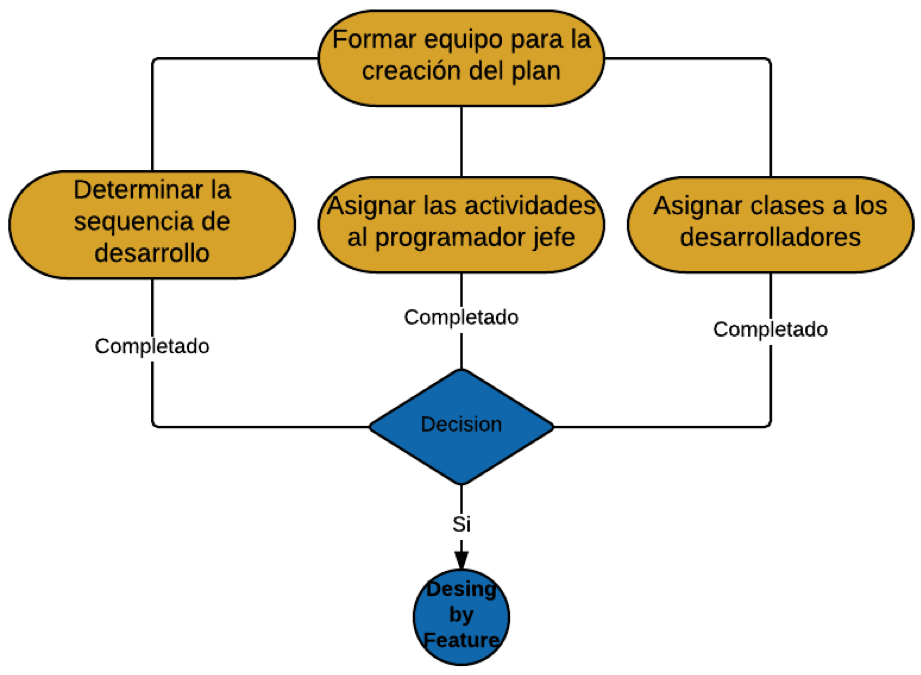
\includegraphics[width=3.8cm]{img/flujo3}
	\caption {Diagrama de flujo de la tercera etapa}
	\label{fig:dcu}
\end{figure}

\subsection{Diseño por característica}
Por cada característica es creado un paquete de diseño, el programador jefe selecciona un pequeño grupo de características,  asignadas previamente, que luego serán desarrolladas.

\subsubsection{Criterio para el inicio de esta etapa}
El plan a sido completado exitosamente.

\subsubsection{Tareas de esta etapa}
\begin{itemize}
	\item Formar al equipo de diseño.
	\item Desarrollar la secuencia de diagramas pertinentes a esta etapa.
	\item Refinar el modelo de objetos.
	\item Inspección del diseño.
\end{itemize}

\subsubsection{Roles participantes de esta etapa}

Programador jefe, equipo de desarrollo, experto de dominio.

\subsubsection{Criterio para el fin de esta etapa}

Creación exitosa y verificada del o los paquetes de diseño.

\subsubsection{Salida}

\begin{itemize}
	\item Diagrama de secuencia.
	\item Modelo de objetos con sus respectivos métodos, atributos y clases.
\end{itemize}

\subsubsection{Diagarama de flujo de trabajo}
\begin{figure}[H]
	\centering
	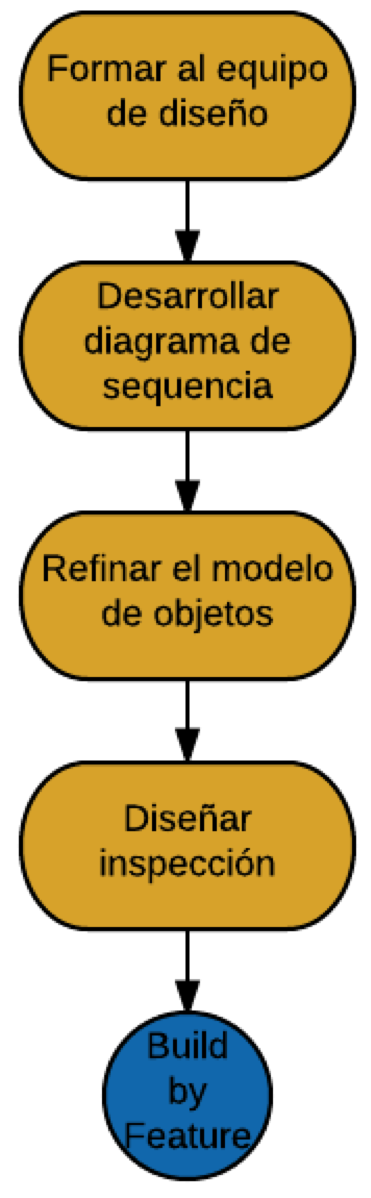
\includegraphics[width=1.5cm]{img/flujo4}
	\caption {Diagrama de flujo de la cuarta etapa}
	\label{fig:dcu}
\end{figure}

\subsection{Construcción de las características}
Trabajando desde los paquetes de diseño, los programadores implementan los elementos necesarios para sus clases. El código desarrollado es probado e inspeccionado.

\subsubsection{Criterio para el inicio de esta etapa}
La etapa de diseño a sido completada con éxito. Los paquetes de diseños han sido inspeccionados correctamente.

\subsubsection{Tareas de esta etapa}
\begin{itemize}
	\item Implementar clases y métodos.
	\item Realizar inspección del código.
	\item Pruebas unitarias.
	\item Aceptación.
	\item Verificación.
\end{itemize}
\subsubsection{Roles participantes de esta etapa}
Programador,Tester.
\subsubsection{Criterio para el fin de esta etapa}
Desarrollo de una o mas características.

\subsubsection{Diagarama de flujo de trabajo}
\begin{figure}[H]
	\centering
	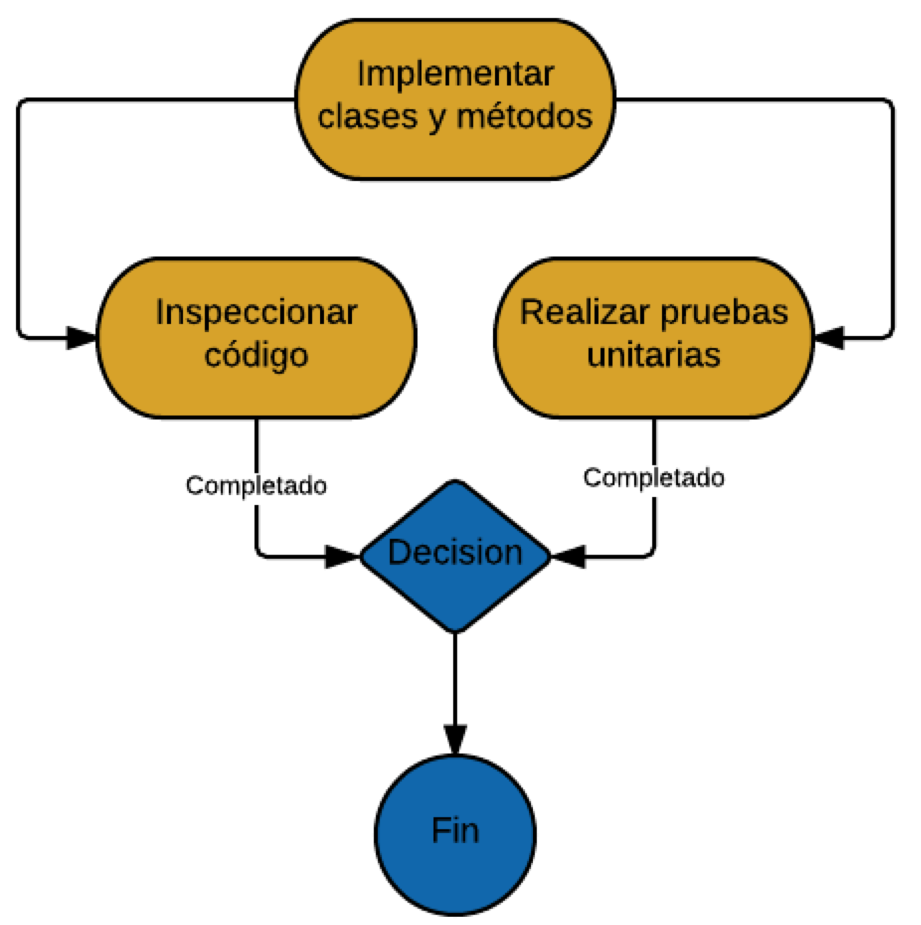
\includegraphics[width=4.5cm]{img/flujo5}
	\caption {Diagrama de flujo de la quinta etapa.}
	\label{fig:dcu}
\end{figure}
\section{Roles y responsabilidades}

\subsubsection{Administrador de proyecto (AP)}
Es el encargado de corroborar el progreso del desarrollo del producto, administrar recursos,  presupuestos y equipamiento.
\subsubsection{Arquitecto jefe (AJ)}
Esta persona posee  habilidades técnicas y de modelamiento, es el responsable de la construcción del modelo general del producto, se encarga de coordinar sesiones en donde el equipo colabora en el diseño del sistema.
\subsubsection{Administrador de desarrollo (AD)}
Es responsable de liderar las actividades diarias de desarrollo. Son requeridas buenas habilidades técnicas. El AD deberá resolver conflictos que el programador jefe no puede abarcar.
\subsubsection{Programador jefe (PJ)}
Este rol corresponde a un desarrollador con experiencia, participando en el levantamiento de requerimientos de alto nivel, analizando y diseñando actividades que serán desarrolladas por pequeños grupos de trabajo.
\subsubsection{Administrador de entregas (AE)}
Se asegura que el programador jefe entregue reportes de progreso cada semana. Estas son informadas directamente al administrador de proyecto.
\subsubsection{Programador (CO)}
Es un miembro de un pequeño grupo de trabajo liderado por el jefe de proyecto. Esta persona diseña, codifica, prueba y documenta las características del sistema en construcción.
\subsubsection{Experto de dominio(ED)}
Corresponde a los usuarios, auspiciadores, analistas de negocio. Los desarrolladores confían en ellos, ya que debido a su conocimiento se asegura la entrega de un producto correcto.

\subsubsection{Diagrama de roles}

\begin{figure}[H]
	\centering
	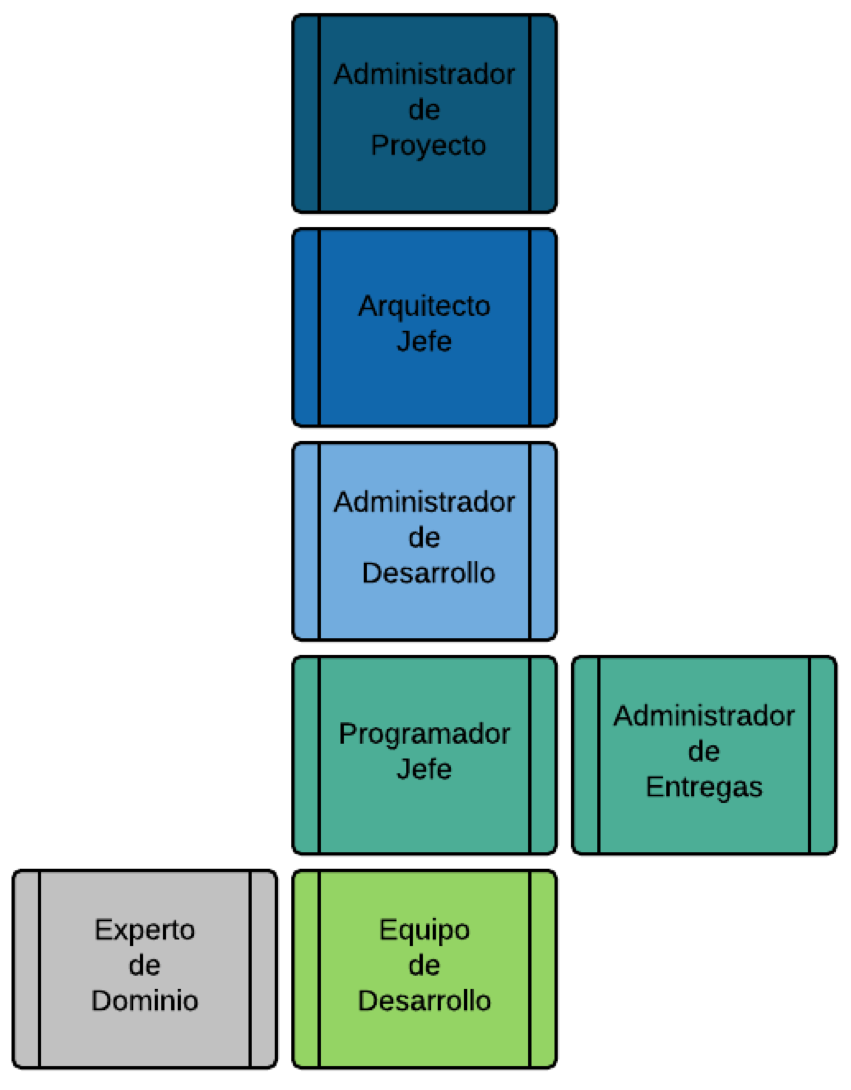
\includegraphics[width=5.5cm]{img/roles}
	\caption {Modelo jerárquico de roles}
	\label{fig:dcu}
\end{figure}

\chapter{Herramientas}

\subsubsection{Herramienta para la administración de proyectos - Gitlab}

\begin{itemize}
	\item Planificación de sprint.
	\item Creación de proyectos.
	\item Distribuir tareas.
\end{itemize}

\subsubsection{Estrategia de bracheo}

El flujo de trabajo se organiza en dos ramas principales, Master y Develop. Ademas existen tres ramas auxiliares Feature, reléase, hotfix [Figura 7.1].

\begin{figure}[H]
	\centering
	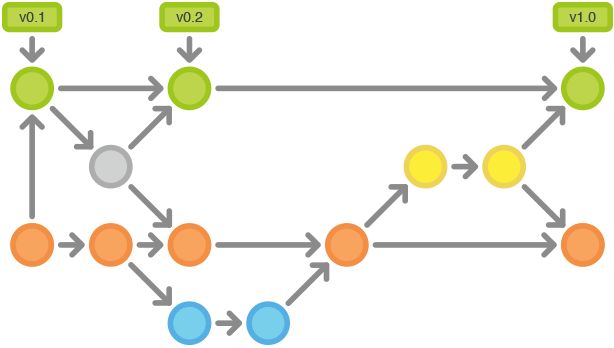
\includegraphics[width=0.3\linewidth]{img/gitflow}
	\caption{Ejemplo de funcionamiento}
	\label{fig:MarcoTeorico}
\end{figure}

\begin{itemize}
	\item Master: Cualquier commit que pongamos en esta rama debe estar listo para ir a producción.
	\item Develop: Aquí se encuentra todo el código asociada a una versión planificada del proyecto.
	\item Feature: Se utilizan para desarrollar nuevas características de la aplicación que, una vez terminadas, se incorporan a la rama develop.
	\item Release: se utilizan para preparar el siguiente código en producción. En estas ramas se hacen los últimos ajustes y se corrigen los últimos bugs antes de pasar el código a producción incorporándolo a la rama master.
	\item Hotfix: Esas ramas se utilizan para corregir errores y bugs en el código en producción (no planificados).
\end{itemize}



\section{Comunicación - Slack}

Esta es una herramienta de mensajería instantánea para equipos, permite tener todas las comunicaciones en un mismo lugar.

\subsubsection{Principales características}

\begin{itemize}
	\item Separación de las comunicaciones en canales, que puede ser públicos o privados.
	\item Integración con GIT.
	\item Facilidad para compartir archivos.
	\item Multiplataforma.
\end{itemize}

\section{Repositorio de contenidos - GIT}

Siendo unas de las mas populares tecnologías de código libre para el control de versiones, Git y Mercurial son muy similares en funcionamiento. Cada archivo modificado es versionado. Para mayor eficiencia estos sistemas de control de versiones no copian archivos sin modificar, en su lugar crean una referencia que apunta a otra versión

\newpage
\section{Gestión del flujo de trabajo - SourceTree}

Source tree es un cliente que permite el uso y seguimiento de repositorios GIT, esta herramienta permite gestionar nuestros proyectos remotos o locales, haciendo uso de una interfaz grafica, tal como podemos apreciar en la [Figura 7.2].

\begin{figure}[H]
	\centering
	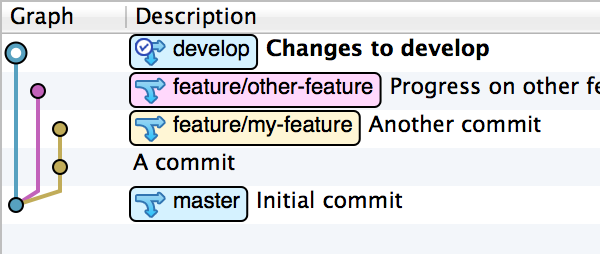
\includegraphics[width=0.4\linewidth]{img/tree.png}
	\caption{Ejemplo de funcionamiento}
	\label{fig:MarcoTeorico}
\end{figure}

\section{Integración continua - Jenkins}

La integración continua es una práctica del desarrollo de software que nace con la aparición de las metodologías ágiles, esta tecnología permite a los miembros de un equipo de trabajo integrar constantemente el código fuente de uno o varios proyectos. Una build es realizada periódicamente para comprobar los cambios, al código fuente, funcionan correctamente antes de ser puestos en los ambientes finales de producción.
Jenkins es un servidor de Integración Continua, gratuito y de código libre basado en tareas, donde se indican las actividades a realizar en una determinada Build. Esta herramienta se enlaza a todo el proceso de desarrollo cuando es importante inspeccionar el código y visualizar resultados de las pruebas unitarias.

\section{Diagrama final de la solución}

\begin{figure}[H]
	\centering
	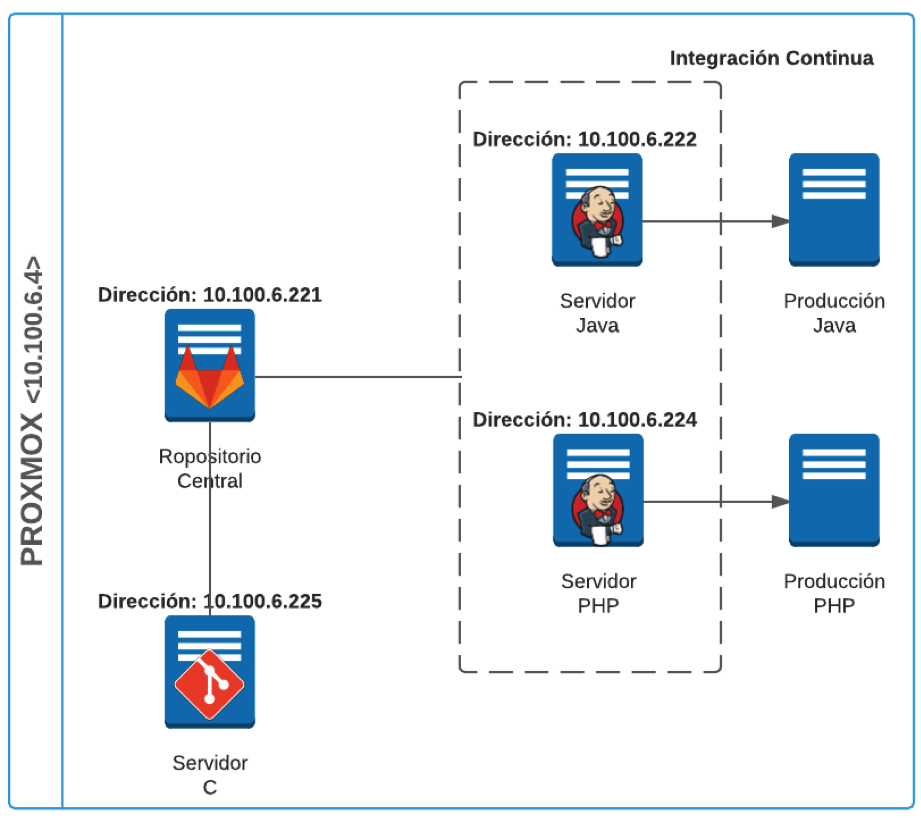
\includegraphics[width=0.3\linewidth]{img/final}
	\caption{Modelo de la solución}
	\label{fig:MarcoTeorico}
\end{figure}

\section{Diseño de pruebas}

En esta sección se muestra la elaboración del tipo de prueba que se utilizara para evaluar la infraestrucutra para el desarrollo colaborativo de software.

\subsection{Pruebas unitarias}

Las pruebas unitarias sirven para aislar modulos del sistema para demostrar su funcionamiento ante un escenario predefinido.
Dado que este sistema corresponde a la integración de diferentes herramientas de código libre, las pruebas seran del tipo caja negra, se especificara de forma previa la entrada y salida de la función a testear.


\begin{table}[htbp]
	\begin{center}
		\begin{tabular}{|l|l|}
			\hline
			Función a probar & Caso de prueba \\
			\hline \hline
			Entrada valida		 &  \\ \hline
			Salida esperada &  \\ \hline
			Entrada invalida &  \\ \hline
			Salida esperada & \\ \hline
			\hline \hline
			Resultado: & \\ \hline
			
		\end{tabular}
		\caption{Modelo general de pruebas.}
		\label{tabla:sencilla}
	\end{center}
\end{table}

\chapter{Implementación}

En este capítulo se presenta la implementación de cada uno de los niveles de la infraestructura de apoyo al desarrollo colaborativo de software con fines docentes, para la integración de prácticas entre asignaturas. 

\section{Hardware de desarrollo}

\subsubsection{Hardware adicional}

\begin{itemize}
	\item \textbf{Nombre}: Macbook Pro, equipo de trabajo del alumno.
	\item \textbf{Sistema Operativo}: OS X El Capitan.
	\item \textbf{CPU}: 2,5 GHz Intel Core i5.
	\item \textbf{Memoria RAM}: 8000MB.
	\item \textbf{HDD}: SATA 2, 500GB.
	
\end{itemize}


\subsubsection{Nivel Físico - Especificaciones del equipo}

\begin{itemize}
	\item \textbf{Nombre}: Nereo, Servidor físico proporcionado por la escuela de Ingeniería  Civil en Informática.
	\item \textbf{Sistema Operativo}: Proxmox Virtual Envirorment v3.4, (Debian Wheezy 7.8).
	\item \textbf{CPU}: Intel(R) Xeon(R) CPU E5504, 2GHz.
	\item \textbf{Memoria RAM}: 4100MB.
	\item \textbf{HDD}: Hitachi SATA HDS721032CLA362 JPFOA39C, 320GB.
	\item \textbf{DVD}: DV-28E-V.
\end{itemize}

\section{Herramientas para el desarrollo}

\subsection{Nivel virtual - Proxmox Virtual Envirorment}

Para esta parte de la implementación fue usado el sistema operativo, de código libre, Proxmox Virtual Envirorment v3.4, como solución de virtualización. 
Proxmox es una herramienta que soporta dos tipos de virtualización, Kernel-Based Virtual Machine (KVM) y Container-Based Virtualization.

OpenVZ permite a un servidor físico ejecutar múltiples instancias aisladas de sistemas operativos, llamados contenedores. Este nucleo modificado provee virtualización, aislamiento y administración de los recursos. Cada maquina virtual posee su propio sistema de archivos, usuarios, red, dispositivos y árbol de procesos. La \textbf{administración de los recursos} funciona en cuatro niveles, estos recursos pueden ser modificados en tiempo de ejecución por lo que no es necesario reiniciar los servidores.

\begin{enumerate}
	\item \textbf{Cuota de disco}: Cada contenedor tiene su propia cuota de disco en bloques de disco e innodes.
	\item \textbf{Planificador de CPU}: Un primer nivel decide a que contenedor le asignara tiempo de CPU, esto en base a los valores de CPU de cada contenedor, en un segundo nivel, decide que proceso ejecutar en ese contenedor.
	\item \textbf{Planificador de entrada y salida}: Basado en la asignación de prioridades de entrada y salida en cada contenedor. El planificador distribuye el ancho de banda disponible acorde a esas prioridades.
	\item \textbf{User Beancounters}: Este nivel asegura que los recursos del sistema no sean monopolizados por un solo contenedor.
	
\end{enumerate}
\newpage
Se configuro la red de Proxmox dentro del segmento de direcciones de la Facultad de Ingeniería de la Universidad de Valparaíso [Figura 9.1].

\begin{figure}[H]
	\centering
	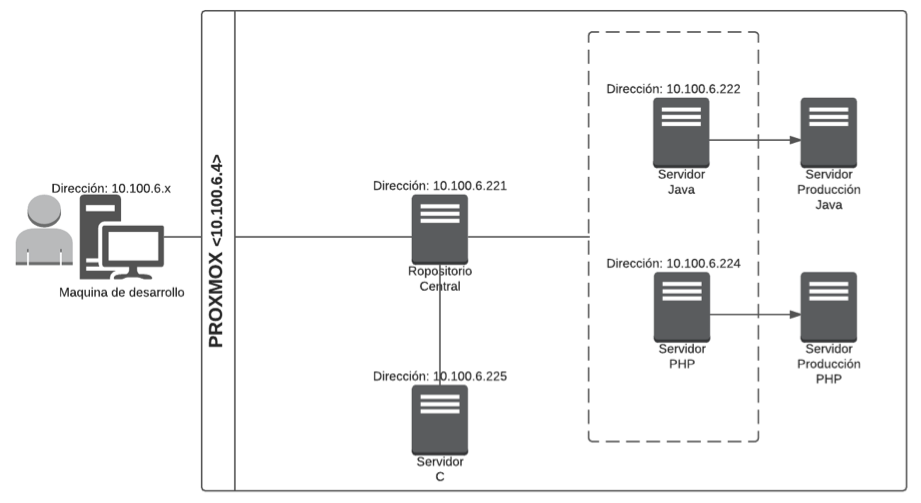
\includegraphics[width=0.6\linewidth]{img/modelodered.png}
	\caption{Modelo de red del sistema}
	\label{fig:MarcoTeorico}
\end{figure}

\subsection{Servidores virtuales - Estructura operacional}

\subsubsection{Repositorio central}

Servidor de administración de repositorios, al cual se conectan los servidores de integración continua y el servidor de desarrollo en C. 
\begin{itemize}
	\item \textbf{Recursos asignados}: RAM @1500MB, HDD 80GB.
	\item \textbf{Red}: Veth device.
	\item \textbf{Sistema operativo}: Ubuntu 14.04 64bits.
	\item \textbf{Paquetes instalados}: Gitlab 8.10.
\end{itemize}

\subsubsection{Servidor Java}

Maquina de integración continua para el desarrollo en lenguaje Java.

\begin{itemize} 
	\item \textbf{Recursos asignados}: RAM @1024MB, HDD 25GB.
	\item \textbf{Red}: Veth device.
	\item \textbf{Dirección IP}: 10.100.6.222.
	\item \textbf{Sistema operativo}: Debian 7.
	\item \textbf{Paquetes instalados}: Jdk 1.8, Maven 3.3, Git 2.7, Jenkins 2.7.
\end{itemize}

\subsubsection{Servidor PHP}

Maquina de integración continua para el desarrollo en lenguaje PHP.

\begin{itemize}
	\item \textbf{Recursos asignados}: RAM @1024MB, HDD 25GB.
	\item \textbf{Red}: Veth device.
	\item \textbf{Dirección IP}: 10.100.6.224.
	\item \textbf{Sistema operativo}: Debian 7.
	\item \textbf{Paquetes instalados}: PHP 5.6, Composer 1.2, Git 2.7, Jenkins 2.7.
\end{itemize}

\subsubsection{Servidor C}

Maquina que permite el desarrollo de programas en lenguaje C.
\begin{itemize}
	\item \textbf{Recursos asignados}: RAM @650MB, HDD 25GB.
	\item \textbf{Red}: Veth device.
	\item \textbf{Dirección IP}: 10.100.6.225.
	\item \textbf{Sistema operativo}: Debian 7.
	\item \textbf{Paquetes instalados}: Git 2.7, Gcc 6.2, Make.
\end{itemize}
\subsubsection{Producción Java}
Servidor de aplicación con la ultima versión del código funcional.

\begin{itemize}
	\item \textbf{Recursos asignados}: RAM @650MB, HDD 25GB.
	\item \textbf{Red}: Veth device.
	\item \textbf{Dirección IP}: 10.100.6.226.
	\item \textbf{Sistema operativo}: Debian 7.
	\item \textbf{Paquetes instalados}: JDK 1.8.
\end{itemize}

\subsubsection{Producción PHP}
Servidor de aplicación con la ultima versión del código funcional.


\begin{itemize}
	\item \textbf{Recursos asignados}: RAM @650MB, HDD 25GB.
	\item \textbf{Red}: Veth device.
	\item \textbf{Dirección IP}: 10.100.6.227.
	\item \textbf{Sistema operativo}: Debian 7.
	\item \textbf{Paquetes instalados}: PHP 5.6.
\end{itemize}

\subsection{Herramientas del sistema - Versión}

Git 2.7: Es un sistema de control de versiones distribuido de código abierto, utilizado en el desarrollo de software y otras tareas. Como sistema distribuido apunta a la velocidad , integración de los datos y soporte al flujo de trabajo distribuido no lineal.

Gitlab 8.11: Es un administrador de repositorios de código libre en donde es posible, tener un seguimiento de las versiones de los repositorios Git. Con esta herramienta es posible el seguimiento de problemas, revisión de código y registro de actividad.

Jenkins 2.19: Es una herramienta, de código libre, para integración continua escrita en Java. Jenkins ejecuta pruebas y construye el código almacenado en el repositorio central.

PHP 5.6: Es un lenguaje de scripting utilizado para construir aplicaciones en el servidor PHP.

PHPunit 5.5.4: Framework para la ejecución de pruebas unitarias para desarrollos en php.

JUnit 4.12: Framework para la ejecución de pruebas unitarias en entornos de desarrollo Java.

Composer 1.2: Es una herramienta para la administración de dependencias en PHP, permite declarar en el archivo composer.json, las librerías que los proyectos necesitan instalar o actualizar de forma automática. 

Jdk 1.8: Plataforma Java, que permite la construcción de aplicaciones en el servidor de desarrollo Java.

Maven 3.3.9: Es una herramienta para la administración de dependencias en Java, permite declarar las librerías que un proyecto necesita instalar de forma automática.

Gcc 6.2: Herramienta de código libre que posee un conjunto de compiladores para el lenguaje C.


\chapter{Vistas}

\section{Proxmox Virtual Envirorment}

Pantalla de acceso a Proxmox VE 3.4 [Figura 10.1]\\

\begin{figure}[H]
	\centering
	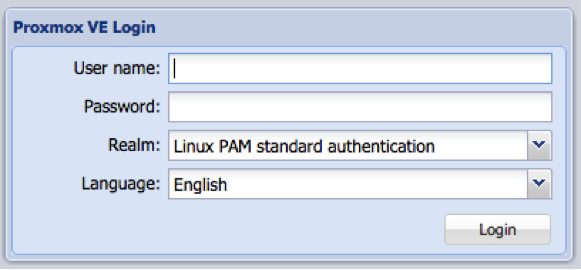
\includegraphics[width=0.3\linewidth]{img/proxmox1.png}
	\caption{Login Proxmox VE}
	\label{fig:MarcoTeorico}
\end{figure}


En la pantalla principal tenemos acceso a la lista de servidores virtuales del nodo pve y pestañas que facilitan la configuración, acceso a información del sistema y graficas del funcionamiento global [Figura 10.2].\\

\begin{figure}[H]
	\centering
	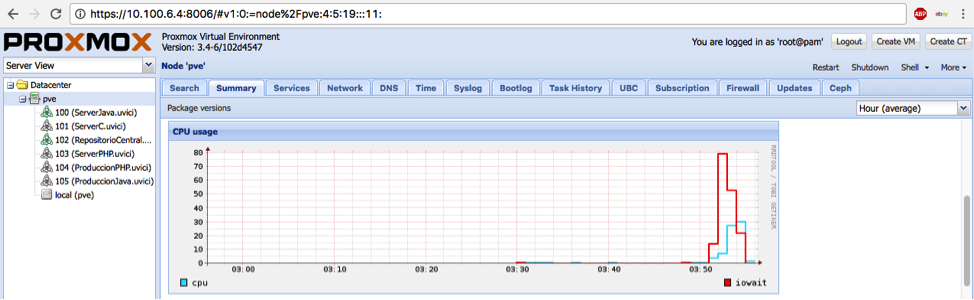
\includegraphics[width=0.6\linewidth]{img/proxmox2.png}
	\caption{Login Proxmox VE}
	\label{fig:MarcoTeorico}
\end{figure}

Los botones create CT/VM permiten crear contenedores y maquinas virtuales almacenadas en el disco del nodo (pve). Desde el disco local podemos subir imágenes y plantillas de otros sistemas operativos [Figura 10.3].\\


\begin{figure}[H]
	\centering
	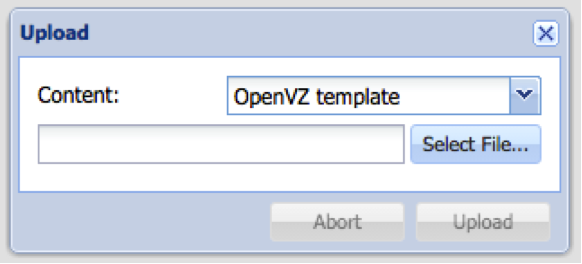
\includegraphics[width=0.3\linewidth]{img/proxmox3.png}
	\caption{Pantalla de carga de imagenes y plantillas}
	\label{fig:MarcoTeorico}
\end{figure}

\section{Gitlab}

Una vez registrados, podemos acceder a la pagina de inicio, en donde es posible seleccionar proyectos o crear nuevos.
El menú lateral ‘Dashboard’ nos permite navegar entre las principales funciones del sistema [Figura 10.4].

\begin{figure}[H]
	\centering
	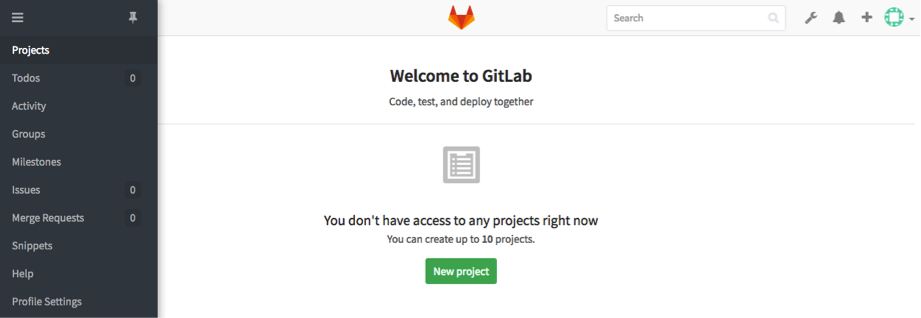
\includegraphics[width=0.5\linewidth]{img/gitlab1.png}
	\caption{Pantalla de inicio Gitlab}
	\label{fig:MarcoTeorico}
\end{figure}

Al presionar sobre el botón ‘New project’ se tiene la siguiente vista [Figura 10.5], desde aquí podemos importar repositorios o crear nuevos.

\begin{figure}[H]
	\centering
	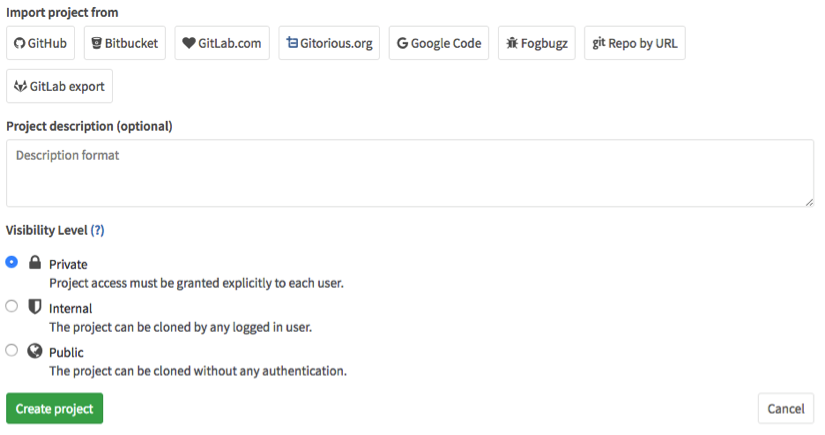
\includegraphics[width=0.4\linewidth]{img/gitlab2.png}
	\caption{Creación nuevo proyecto}
	\label{fig:MarcoTeorico}
\end{figure}


Dentro de un proyecto [Figura 10.6], es posible tener acceso a sus  archivos y actividad.

\begin{figure}[H]
	\centering
	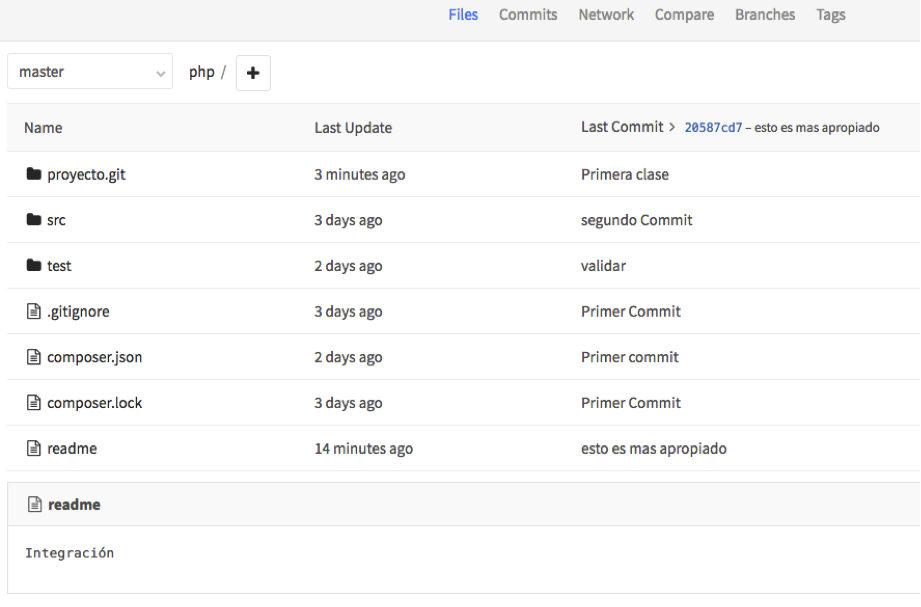
\includegraphics[width=0.7\linewidth]{img/gitlab3.png}
	\caption{Creación nuevo proyecto}
	\label{fig:MarcoTeorico}
\end{figure}

Desde la pestaña Network es posible acceder a la línea de tiempo del proyecto, aquí podemos volver a una versión anterior del trabajo o movernos a una mas reciente [Figura 10.7].

\begin{figure}[H]
	\centering
	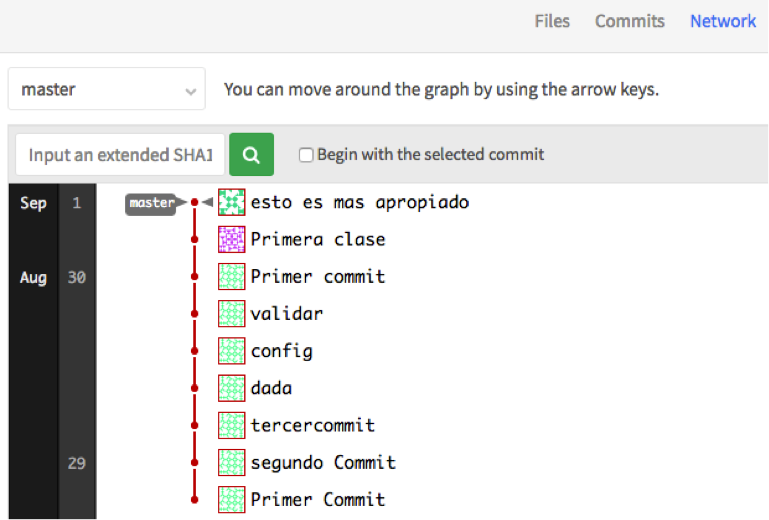
\includegraphics[width=0.7\linewidth]{img/gitlab4.png}
	\caption{Creación nuevo proyecto}
	\label{fig:MarcoTeorico}
\end{figure}

Para incorporar colaboradores a un proyecto, el creador debe agregar las llaves publicas de los miembros del equipo (idrsa.pub), en su perfil de usuario [Figura 10.8].

\begin{figure}[H]
	\centering
	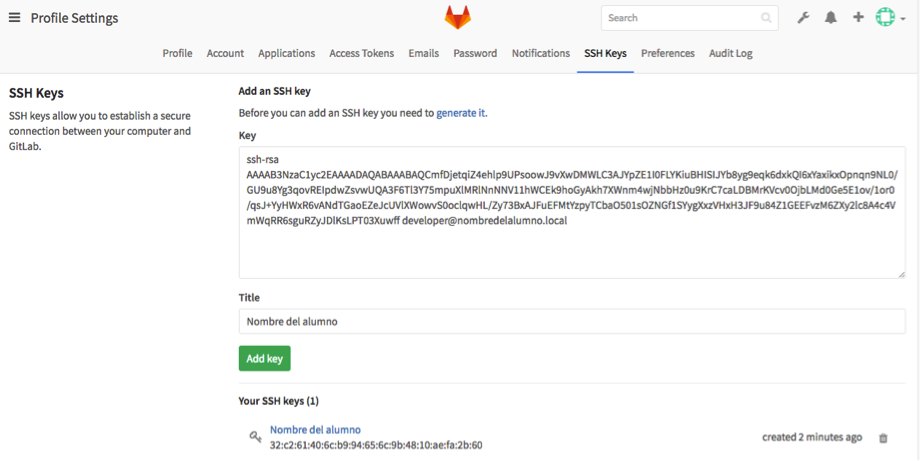
\includegraphics[width=1.15\linewidth]{img/gitlab5.png}
	\caption{Creación nuevo proyecto}
	\label{fig:MarcoTeorico}
\end{figure}

\section{Jenkins}

Para acceder a la pantalla de inicio de Jenkins debemos llenar los campos usuario y contraseña [Figura 10.9].

\begin{figure}[H]
	\centering
	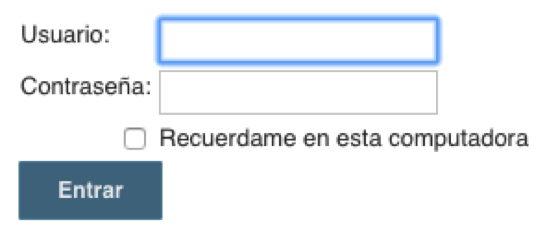
\includegraphics[width=0.3\linewidth]{img/jenkins1.png}
	\caption{Login Jenkins}
	\label{fig:MarcoTeorico}
\end{figure}

La pantalla principal del sistema es como se muestra [Figura 10.10], desde aquí es posible configurar, tener acceso y crear nuevas tareas (Proyecto-php).

\begin{figure}[H]
	\centering
	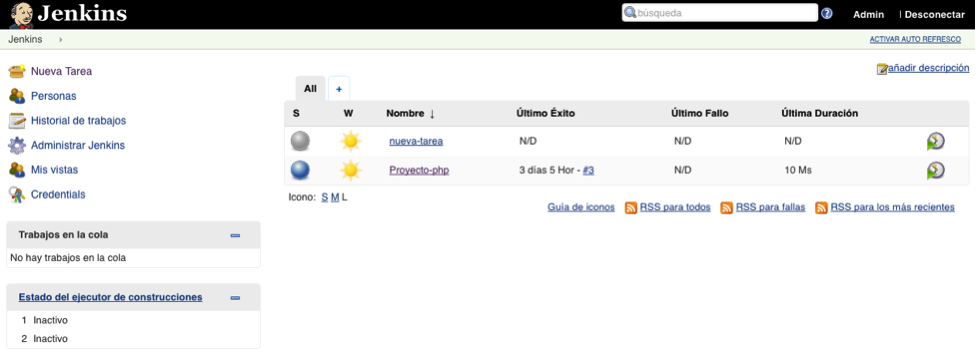
\includegraphics[width=0.8\linewidth]{img/jenkins2.png}
	\caption{Pantalla de inicio Jenkins}
	\label{fig:MarcoTeorico}
\end{figure}

Con el botón nueva tarea permite configurar la integración de nuevos proyectos [Figura 10.11], aquí es posible especificar el repositorio, triggers y pasos de construcción.

\begin{figure}[H]
	\centering
	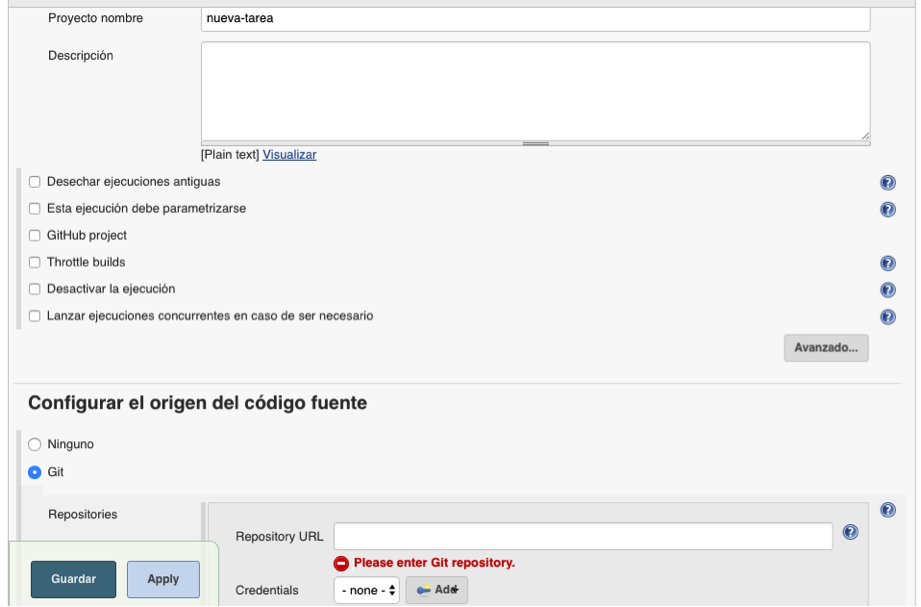
\includegraphics[width=0.9\linewidth]{img/jenkins3.png}
	\caption{Crear/Configurar proyecto}
	\label{fig:MarcoTeorico}
\end{figure}

Desde el menú build step podemos agregar comandos (probar, instalar, compilar) para que sean ejecutados por Jenkins [Figura 10.12].
\begin{figure}[H]
	\centering
	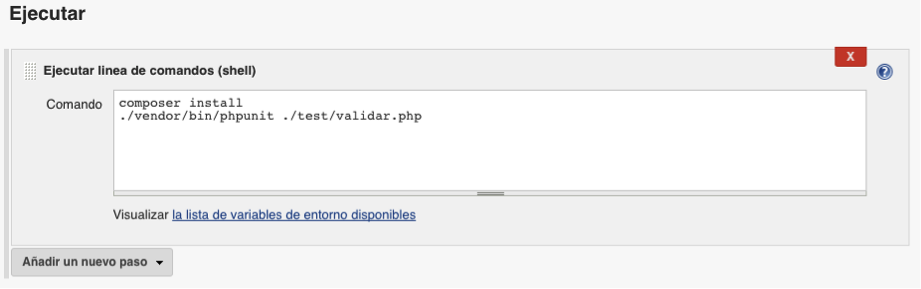
\includegraphics[width=0.7\linewidth]{img/jenkins4.png}
	\caption{Crear/Configurar proyecto}
	\label{fig:MarcoTeorico}
\end{figure}



Una vez creado y configurado un proyecto es posible ejecutar manualmente su construcción.  Se tiene una copia de los archivos de la ultima build dentro del espacio de trabajo de Jenkins, en el historial de tareas tiene el registro de las ultimas build creadas, azul indica que el proceso fue exitoso [Figura 10.13].

\begin{figure}[H]
	\centering
	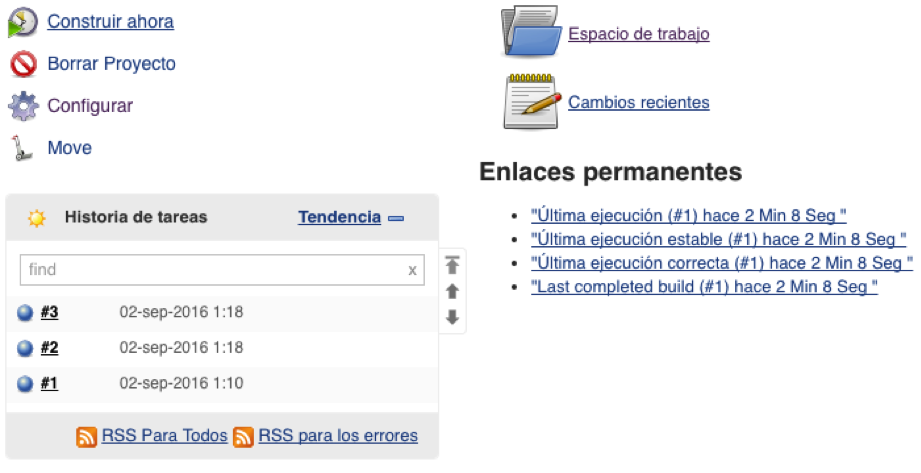
\includegraphics[width=0.5\linewidth]{img/jenkins5.png}
	\caption{Construir proyecto}
	\label{fig:MarcoTeorico}
\end{figure}

Al seleccionar una build del menú ‘Historia de tareas’ [Figura 10.14] podemos acceder a su salida de consola.

\begin{figure}[H]
	\centering
	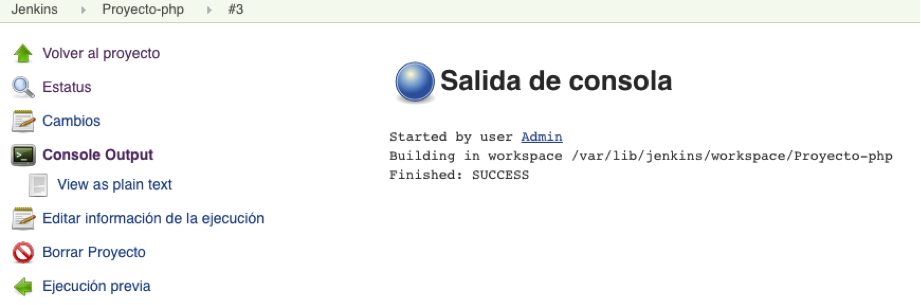
\includegraphics[width=0.6\linewidth]{img/jenkins6.png}
	\caption{Salida de consola}
	\label{fig:MarcoTeorico}
\end{figure}



El uso del sistema es como se muestra en la Figura, en el contexto de la utilización de la metodología ágil ‘Feature Driven Development’, se tendría el siguiente flujo de trabajo.

Primero un grupo de usuarios, trabaja en el desarrollo de una característica, con tiempo de implementación menor a dos días, estos desarrolladores hacen push (envían cambios al repositorio central) de sus últimas versiones. 
Luego el servidor de integración continua, Java o PHP, automáticamente ejecuta los test a las clases y construye una Build de la ultima versión del Master branch, esto a través de la configuración de un trigger, si todas las pruebas son superadas, el servidor de integración continua se encarga de mover los archivos al ambiente de producción que corresponda.


\begin{figure}[H]
	\centering
	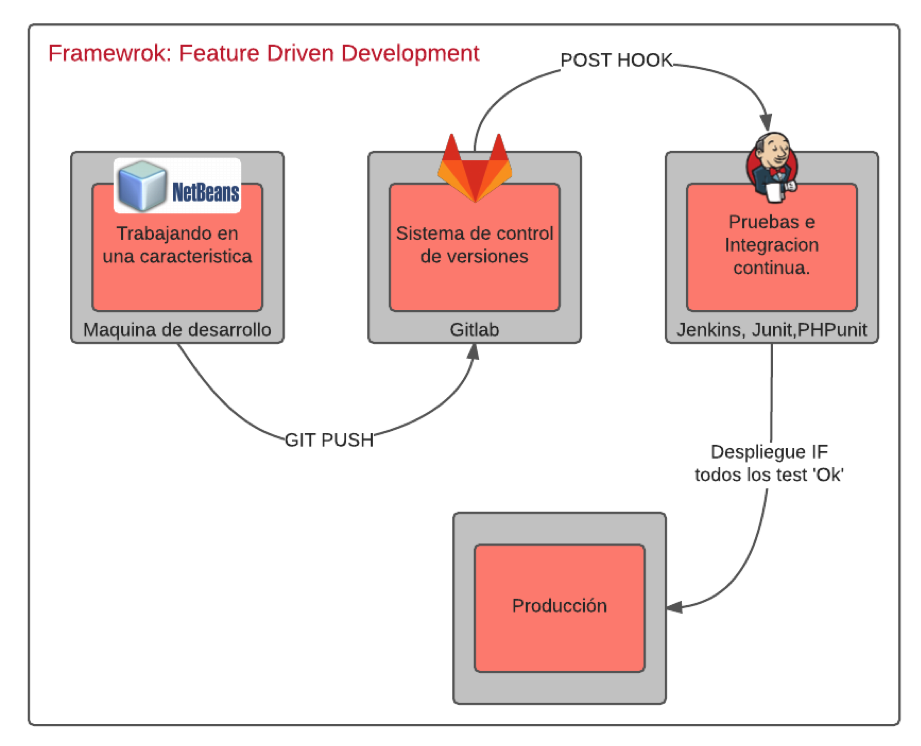
\includegraphics[width=0.5\linewidth]{img/flujo.png}
	\caption{Flujo general del sistema}
	\label{fig:MarcoTeorico}
\end{figure}


\section{Navegabilidad del sistema}

Cada unos de los sistemas navegables de esta solución son accedidos de manera independiente, a traves del browser del usuario.

\subsection{Proxmox}

\begin{figure}[H]
	\centering
	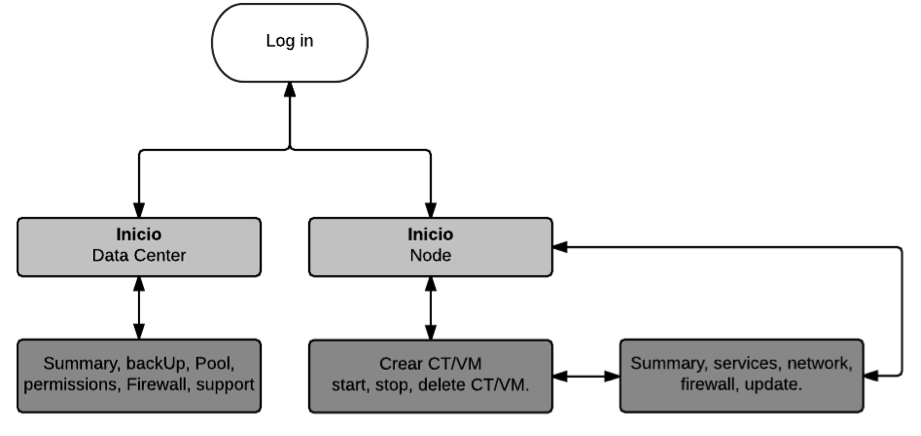
\includegraphics[width=0.4\linewidth]{img/proxmoxnav.png}
	\caption{Diagrama de navegabilidad de la web GUI de Proxmox}
	\label{fig:MarcoTeorico}
\end{figure}

\subsection{Gitlab}

\begin{figure}[H]
	\centering
	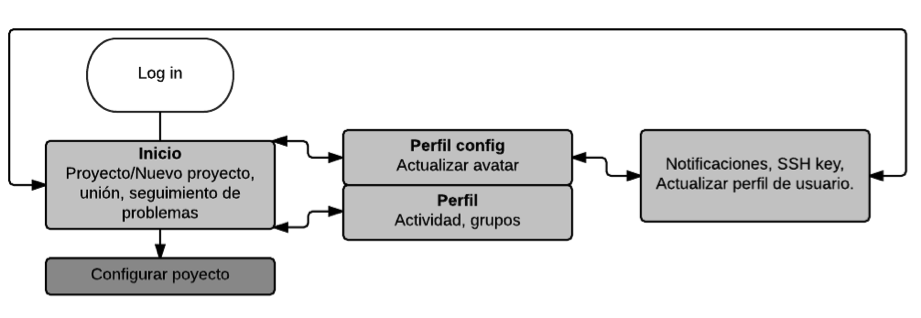
\includegraphics[width=0.4\linewidth]{img/gitlabnav.png}
	\caption{Diagrama de navegabilidad de la web GUI de Gitlab}
	\label{fig:MarcoTeorico}
\end{figure}

\subsection{Jenkins}

\begin{figure}[H]
	\centering
	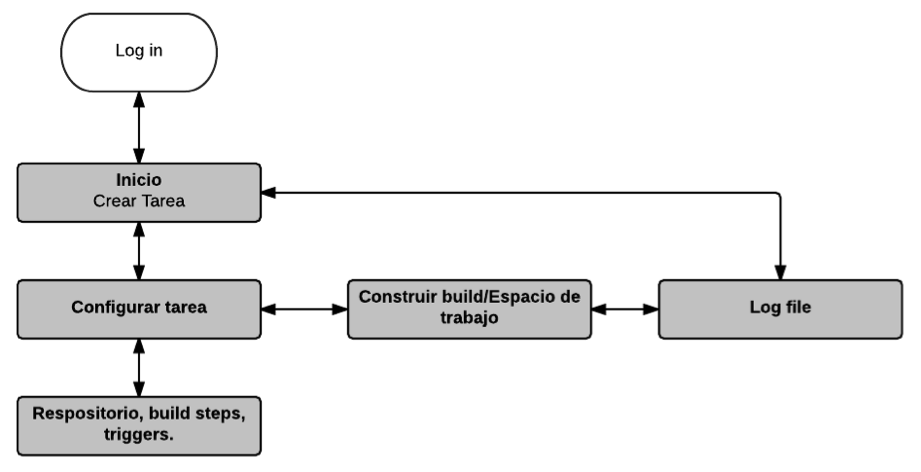
\includegraphics[width=0.4\linewidth]{img/jenkinsnav.png}
	\caption{Diagrama de navegabilidad de la web GUI de Jenkins}
	\label{fig:MarcoTeorico}
\end{figure}

\chapter{Pruebas}

\subsubsection{Nivel de las pruebas}

\begin{itemize}
	\item Pruebas de requerimientos: Primero se verifican los los requerimientos y luego se comprueba que el sistema los satisfaga correctamente.
	\item Pruebas funcionales y de sistema: Usando tecnicas de pruebas del tipo caja negra, se busca determinar si la funcionalidad especificada en el requerimiento opera correctamente.
	\item Pruebas de validación: Mediante un ejemplo de funcionamiento se verifica el cumplimiento de las especificaciones del sistema y si este logra el próposito pora el cual fue diseñado.
\end{itemize}

\section{Pruebas de requerimientos}

Los resultados de la prueba de requerimientos se presentan en la Tabla 10.1, en donde se visualiza que se cumplen los item en su totalidad.
La Tabla 10.1 muestra la lista de requerimientos, en donde es posible apreciar el cumplimiento de los Items.

\begin{table}[H]
	\begin{center}
		\begin{tabular}{| p{7cm} | p{2cm} | p{2cm} |}
			\hline
			Pregunta & SI & NO \\
			\hline \hline
			¿El Documento se adhiere a los estandares? & X &  \\ \hline
			Claridad & X &  \\ \hline
			¿La espeficicación es clara y facil de entender? & X &  \\ \hline
			¿Se refleja el comportamiento del sistema? &  & X \\ \hline
			¿Estan Especificados los requerimientos? & X &  \\ \hline
			¿Los requerimientos ayudan a cumplir el propostito del sistema? & X &  \\ \hline
		\end{tabular}
		\caption{Tabla de evaluación de requerimientos}
		\label{tabla:sencilla}
	\end{center}
\end{table}

\begin{table}[H]
	\begin{center}
		\begin{tabular}{|l|l|}
			\hline
			Identificador & Estado  \\
			\hline \hline
			RF1		 &  Completado \\ \hline
			RF2		 &  Completado \\ \hline
			RF3		 &  Completado \\ \hline
			RF4		 &  Completado \\ \hline
			RF5		 &  Completado  \\  \hline
			RF6		 &  Completado \\ \hline
			RF7		 &  Completado \\ \hline
			RF8		 &  Completado \\ \hline
			\hline \hline
			Total item: & 8/8\\ \hline
			
		\end{tabular}
		\caption{Lista de requerimientos}
		\label{tabla:sencilla}
	\end{center}
\end{table}
\newpage
\section{Pruebas funcionales}

Las Pruebas fueron realizadas bajo el principio de caja negra [Figura 10.1], testers examinan en un alto nivel el diseño y los requerimientos para planear los casos de prueba, se busca asegurar funcionamiento del modulo. De esta manera se examinan  las salidas del sistema, sin importar el funcionamiento interno del modulo inspeccionado.

\begin{figure}[H]
	\centering
	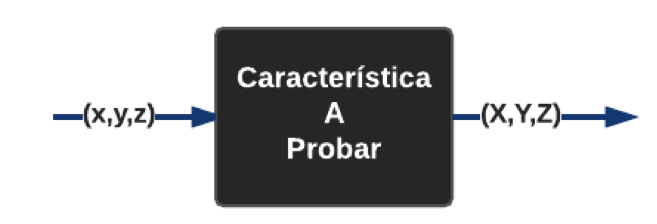
\includegraphics[width=0.7\linewidth]{img/cajanegra.png}
	\caption{Diagrama de entrada y salida}
	\label{fig:MarcoTeorico}
\end{figure}
En esta etapa de la evaluación se hara uso de una métrica [Tabla 10.2] que facilite identificar el origen de un resultado incorrecto o inesperado.

\begin{table}[htbp]
	\begin{center}
		\begin{tabular}{| p{3cm} | p{7cm} | p{1cm} |}
			\hline
			Resultado & Definición & Sigla \\
			\hline \hline
			Error Humano & Acción Humana que produce un resultado incorrecto & M \\ \hline
			Defecto & Paso, proceso o definición de datos incorrecto & D \\ \hline
			Falla &la incapacidad de un componente para realizar la función requerida
			dentro de los requisitos de funcionamiento especificados.  & F \\ \hline
			Error & Diferencia entre el valor medido y el teorico & E \\ \hline
			No aplica & Sin hallazgos & n/a \\ \hline
		\end{tabular}
		\caption{Métricas de evaluación}
		\label{tabla:sencilla}
	\end{center}
\end{table}
\newpage

\subsection{Detalle de las pruebas funcionales}

A continuación se presentan los diagramas de prueba y resultados de la evaluación del sistema.

\subsubsection{Prueba funcional 01}

\begin{figure}[H]
	\centering
	\includegraphics[width=0.5\linewidth]{img/p01.png}
	\caption{Diagrama de entrada y salida}
	\label{fig:MarcoTeorico}
\end{figure}

\begin{table}[H]
	\centering
	\begin{tabular}{  >{\centering\arraybackslash}m{0.5cm} >{\centering\arraybackslash}m{3cm}  >{\arraybackslash}m{4cm}  >{\arraybackslash}m{4cm}  >{\centering\arraybackslash}m{4cm} }
		\hline
		ID & Escenario & Caso de prueba & Entrada & Salida esperada\\
		\hline \hline
		01.1& Iniciar sesión Gitlab & Ingreso de campos usuario y contraseña correctos & Usuario:'almunoiciuv', Password: alumnoiciuv & El Usuario Inicia Sesión\\
		\hline
	\end{tabular}
	\caption{Resumen de resultados}
	\label{tabla:autores}
\end{table}

\begin{table}[H]
	\centering
	\begin{tabular}{  >{\centering\arraybackslash}m{0.5cm} >{\centering\arraybackslash}m{3cm}  >{\arraybackslash}m{4cm}  >{\arraybackslash}m{4cm}  >{\centering\arraybackslash}m{4cm} }
		\hline
		ID & Escenario & Caso de Prueba & Entrada & Salida Esperada\\
		\hline \hline
		01.2 & Iniciar sesión Gitlab & Ingreso del campo usuario incorrecto & Usuario:'almunouvici', Password:'alumnouvici' & Error al iniciar sesión\\
		\hline \hline
		01.2 & Iniciar Sesión Gitlab & Ingreso del campo contraseña incorrecto & Usuario:'almunoiciuv', Password:'alumnouvici' & Error al iniciar sesión\\
		\hline
	\end{tabular}
	\caption{Resumen de resultados}
	\label{tabla:autores}
\end{table}

\begin{table}[H]
	\centering
	\begin{tabular}{  >{\centering\arraybackslash}m{0.5cm} >{\centering\arraybackslash}m{3cm}  >{\arraybackslash}m{4cm}  >{\arraybackslash}m{4cm}  >{\centering\arraybackslash}m{4cm} }
		\hline
		ID & Escenario & Caso de prueba & Entrada & Salida esperada\\
		\hline \hline
		01.3& Iniciar sesión Gitlab & Campo Usuario Vacio & Password:alumnouvici & El sistema indica que el campo Usuario se encuentra vacio.\\
		\hline
		01.3& Iniciar sesión Gitlab & Campo Usuario Vacio & Usuario:alumnouvici : & El sistema indica que el campo Usuario se encuentra vacio.\\
		\hline
		01.3& Iniciar sesión Gitlab & Campo Usuario y Contraseña Vacio & vacio & El sistema indica que el campo Uuuario se encuentra vacio.\\
		\hline
	\end{tabular}
	\caption{Resumen de resultados}
	\label{tabla:autores}
\end{table}


\subsubsection{Prueba funcional 02}

\begin{figure}[H]
	\centering
	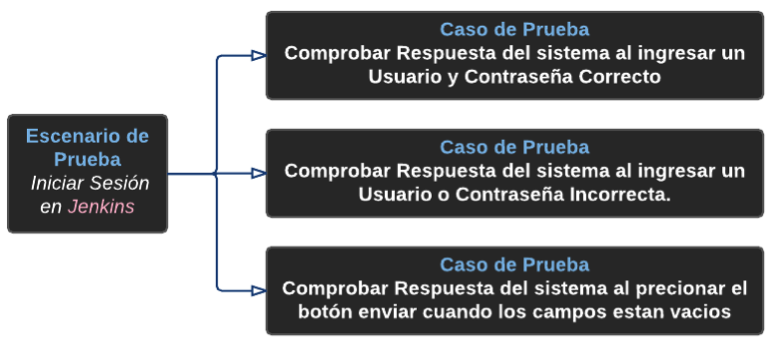
\includegraphics[width=0.555\linewidth]{img/p02.png}
	\caption{Diagrama de entrada y salida}
	\label{fig:MarcoTeorico}
\end{figure}

\begin{table}[H]
	\centering
	\begin{tabular}{  >{\centering\arraybackslash}m{0.5cm} >{\centering\arraybackslash}m{3cm}  >{\arraybackslash}m{4cm}  >{\arraybackslash}m{4cm}  >{\centering\arraybackslash}m{4cm} }
		\hline
		ID & Escenario & Caso de prueba & Entrada & Salida esperada\\
		\hline \hline
		02.1& Iniciar sesión Jenkins & Ingreso de campos usuario y contraseña correctos & Usuario:'almunoiciuv', Password: alumnoiciuv & El usuario inicia sesión\\
		\hline
	\end{tabular}
	\caption{Resumen de resultados}
	\label{tabla:autores}
\end{table}

\begin{table}[H]
	\centering
	\begin{tabular}{  >{\centering\arraybackslash}m{0.5cm} >{\centering\arraybackslash}m{3cm}  >{\arraybackslash}m{4cm}  >{\arraybackslash}m{4cm}  >{\centering\arraybackslash}m{4cm} }
		\hline
		ID & Escenario & Caso de prueba & Entrada & Salida esperada\\
		\hline \hline
		02.2 & Iniciar sesión Jenkins & Ingreso del campo usuario incorrecto & Usuario:'almunouvici', Password:'alumnouvici' & Error al iniciar sesión\\
		\hline \hline
		02.2 & Iniciar sesión Jenkins & Ingreso del campo contraseña incorrecto & Usuario:'almunoiciuv', Password:'alumnouvici' & Error al iniciar sesión\\
		02.2 & Iniciar sesión Jenkins & Ingreso ambos campos incorrectos & Usuario:'almunouv', Password:'alumnouv' & Error al iniciar sesión\\
		\hline
	\end{tabular}
	\caption{Resumen de resultados}
	\label{tabla:autores}
\end{table}

\begin{table}[H]
	\centering
	\begin{tabular}{  >{\centering\arraybackslash}m{0.5cm} >{\centering\arraybackslash}m{3cm}  >{\arraybackslash}m{4cm}  >{\arraybackslash}m{4cm}  >{\centering\arraybackslash}m{4cm} }
		\hline
		ID & Escenario & Caso de prueba & Entrada & Salida esperada\\
		\hline \hline
		02.3& Iniciar sesión Jenkins & Campo usuario vacio & Password: alumnouvici  & El sistema indica que el campo usuario se encuentra vacio.\\
		\hline
		02.3& Iniciar Sesión Jenkins & Campo Usuario Vacio & Usuario: alumnouvici& El sistema indica que el campo usuario se encuentra vacio.\\
		\hline
		02.3& Iniciar sesión Jenkins & Campo usuario y contraseña Vacio & vacio & El sistema indica que el campo usuario se encuentra vacio.\\
		\hline
	\end{tabular}
	\caption{Resumen de resultados}
	\label{tabla:autores}
\end{table}


\subsubsection{Prueba funcional 03}

\begin{figure}[H]
	\centering
	\includegraphics[width=0.55\linewidth]{img/prox.png}
	\caption{Diagrama de entrada y salida}
	\label{fig:MarcoTeorico}
\end{figure}

\begin{table}[H]
	\centering
	\begin{tabular}{  >{\centering\arraybackslash}m{0.5cm} >{\centering\arraybackslash}m{3cm}  >{\arraybackslash}m{4cm}  >{\arraybackslash}m{4cm}  >{\centering\arraybackslash}m{4cm} }
		\hline
		ID & Escenario & Caso de prueba & Entrada & Salida esperada\\
		\hline \hline
		03.1& Iniciar sesión Proxmox & Ingreso de campos usuario y contraseña correctos & Usuario:'root', Password: adminici & El usuario Inicia sesión\\
		\hline
	\end{tabular}
	\caption{Resumen de resultados}
	\label{tabla:autores}
\end{table}

\begin{table}[H]
	\centering
	\begin{tabular}{  >{\centering\arraybackslash}m{0.5cm} >{\centering\arraybackslash}m{3cm}  >{\arraybackslash}m{4cm}  >{\arraybackslash}m{4cm}  >{\centering\arraybackslash}m{4cm} }
		\hline
		ID & Escenario & Caso de prueba & Entrada & Salida esperada\\
		\hline \hline
		03.2 & Iniciar sesión Proxmox & Ingreso del campo Usuario incorrecto & Usuario:'rot', Password:'adminici' & Error al iniciar sesión\\
		\hline \hline
		03.2 & Iniciar sesión Proxmox & Ingreso del campo contraseña incorrecto & Usuario:'root', Password:'iciadmin' & Error al iniciar sesión\\
		03.2 & Iniciar sesión Proxmox & Ambos campos incorrectos & Usuario:'root', Password:'iciadmin' & Error al iniciar sesión\\
		\hline
	\end{tabular}
	\caption{Resumen de resultados}
	\label{tabla:autores}
\end{table}

\begin{table}[H]
	\centering
	\begin{tabular}{  >{\centering\arraybackslash}m{0.5cm} >{\centering\arraybackslash}m{3cm}  >{\arraybackslash}m{4cm}  >{\arraybackslash}m{4cm}  >{\centering\arraybackslash}m{4cm} }
		\hline
		ID & Escenario & Caso de prueba & Entrada & Salida esperada\\
		\hline \hline
		03.3& Iniciar sesión en Proxmox & Campo Usuario vacio & Password: alumnouvici  & El sistema indica que el campo usuario se encuentra vacio.\\
		\hline
		03.3& Iniciar sesión Promox & Campo usuario vacio & Usuario: alumnouvici & El sistema indica que el campo usuario se encuentra vacio.\\
		\hline
		03.3& Iniciar sesión Proxmox & Campo usuario y Contraseña Vacio & vacio  & El sistema indica que el campo usuario se encuentra vacio.\\
		\hline
	\end{tabular}
	\caption{Resumen de resultados}
	\label{tabla:autores}
\end{table}



\subsubsection{Prueba funcional 04}

\begin{figure}[H]
	\centering
	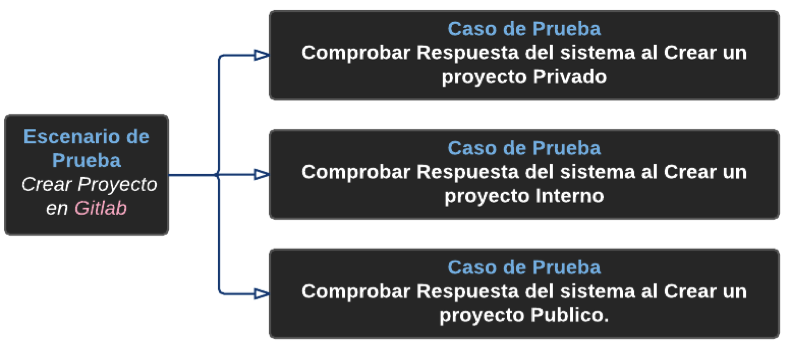
\includegraphics[width=0.55\linewidth]{img/p03.png}
	\caption{Diagrama de entrada y salida}
	\label{fig:MarcoTeorico}
\end{figure}

\begin{table}[H]
	\centering
	\begin{tabular}{  >{\centering\arraybackslash}m{0.5cm} >{\centering\arraybackslash}m{3cm}  >{\arraybackslash}m{4cm}  >{\arraybackslash}m{4cm}  >{\centering\arraybackslash}m{4cm} }
		\hline
		ID & Escenario & Caso de prueba & Entrada & Salida esperada\\
		\hline \hline
		04.1& Crear proyecto en Gitlab & Crear proyecto privado & Nombre: ProyectoPrivado & Proyecto creado\\
		\hline
	\end{tabular}
	\caption{Resumen de resultados}
	\label{tabla:autores}
\end{table}

\begin{table}[H]
	\centering
	\begin{tabular}{  >{\centering\arraybackslash}m{0.5cm} >{\centering\arraybackslash}m{3cm}  >{\arraybackslash}m{4cm}  >{\arraybackslash}m{4cm}  >{\centering\arraybackslash}m{4cm} }
		\hline
		ID & Escenario & Caso de prueba & Entrada & Salida esperada\\
		\hline \hline
		04.2& Crear proyecto en Gitlab & Crear proyecto interno & Nombre: ProyectoInterno & Proyecto creado\\
		\hline
	\end{tabular}
	\caption{Resumen de resultados}
	\label{tabla:autores}
\end{table}

\begin{table}[H]
	\centering
	\begin{tabular}{  >{\centering\arraybackslash}m{0.5cm} >{\centering\arraybackslash}m{3cm}  >{\arraybackslash}m{4cm}  >{\arraybackslash}m{4cm}  >{\centering\arraybackslash}m{4cm} }
		\hline
		ID & Escenario & Caso de prueba & Entrada & Salida esperada\\
		\hline \hline
		04.3& Crear proyecto en Gitlab & Crear proyecto publico & Nombre: ProyectoPublico & Proyecto creado\\
		\hline
	\end{tabular}
	\caption{Resumen de resultados}
	\label{tabla:autores}
\end{table}

\subsubsection{Prueba Funcional 05}

\begin{figure}[H]
	\centering
	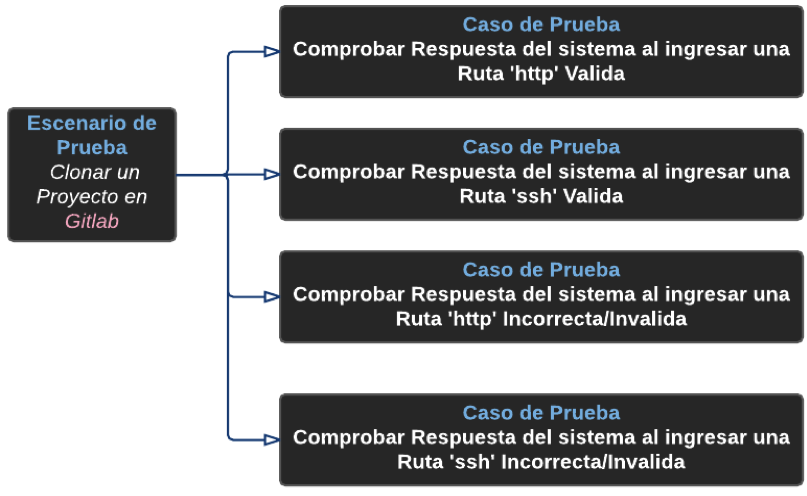
\includegraphics[width=0.55\linewidth]{img/p04.png}
	\caption{Diagrama de entrada y salida}
	\label{fig:MarcoTeorico}
\end{figure}

\begin{table}[H]
	\centering
	\begin{tabular}{  >{\centering\arraybackslash}m{0.5cm} >{\centering\arraybackslash}m{3cm}  >{\arraybackslash}m{4cm}  >{\arraybackslash}m{4cm}  >{\centering\arraybackslash}m{4cm} }
		\hline
		ID & Escenario & Caso de prueba & Entrada & Salida esperada\\
		\hline \hline
		05.1& Clonar un proyecto & Clonar usando una ruta 'http' Valida & http://RepoCentral.uvici/root/php-proyecto-ci.git &  Los archivos asociados al proyecto son recibidos correctamente\\
		\hline
	\end{tabular}
	\caption{Resumen de resultados}
	\label{tabla:autores}
\end{table}
\begin{table}[H]
	\centering
	\begin{tabular}{  >{\centering\arraybackslash}m{0.5cm} >{\centering\arraybackslash}m{3cm}  >{\arraybackslash}m{4cm}  >{\arraybackslash}m{4cm}  >{\centering\arraybackslash}m{4cm} }
		\hline
		ID & Escenario & Caso de prueba & Entrada & Salida esperada\\
		\hline \hline
		05.2& Clonar un proyecto & Clonar usando una ruta 'ssh' Valida & git@RepoCentral.uvici:root/php-proyecto-ci.git &  Los archivos asociados al proyecto son recibidos correctamente\\
		\hline
	\end{tabular}
	\caption{Resumen de resultados}
	\label{tabla:autores}
\end{table}
\begin{table}[H]
	\centering
	\begin{tabular}{  >{\centering\arraybackslash}m{0.5cm} >{\centering\arraybackslash}m{3cm}  >{\arraybackslash}m{4cm}  >{\arraybackslash}m{4cm}  >{\centering\arraybackslash}m{4cm} }
		\hline
		ID & Escenario & Caso de prueba & Entrada & Salida esperada\\
		\hline \hline
		05.3& Clonar un proyecto & Clonar un proyecto Usando una ruta 'http' incorrecta & http://10.100.6221/root/php-proyecto-ci.git &  Los archivos asociados al proyecto son recibidos correctamente.\\
		\hline
	\end{tabular}
	\caption{Resumen de resultados}
	\label{tabla:autores}
\end{table}

\begin{table}[H]
	\centering
	\begin{tabular}{  >{\centering\arraybackslash}m{0.5cm} >{\centering\arraybackslash}m{3cm}  >{\arraybackslash}m{4cm}  >{\arraybackslash}m{4cm}  >{\centering\arraybackslash}m{4cm} }
		\hline
		ID & Escenario & Caso de prueba & Entrada & Salida esperada\\
		\hline \hline
		05.4& Clonar un proyecto & Clonar un proyecto Usando una ruta 'http' Incorrecta & http://10.100.6.221/root/php-proyecto-ci.git &  Los archivos asociados al proyecto son recibidos correctamente.\\
		\hline
	\end{tabular}
	\caption{Resumen de resultados}
	\label{tabla:autores}
\end{table}


\subsubsection{Prueba funcional 06}

\begin{figure}[H]
	\centering
	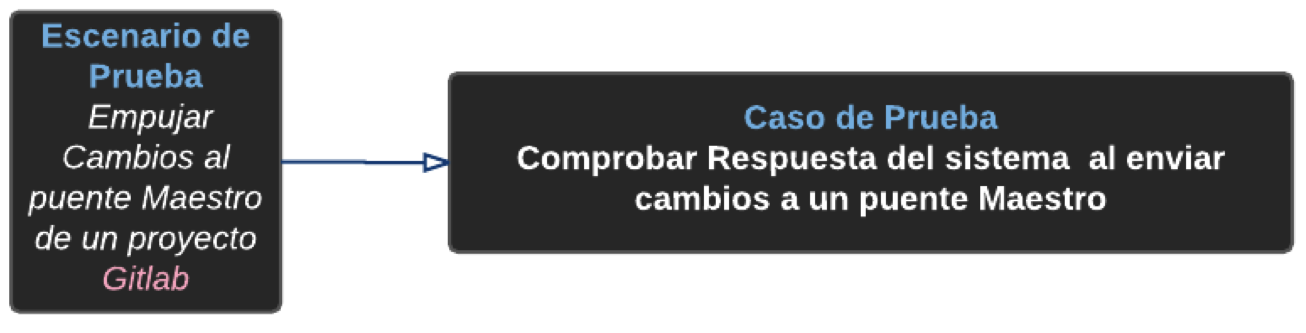
\includegraphics[width=0.55\linewidth]{img/p05.png}
	\caption{Diagrama de entrada y salida}
	\label{fig:MarcoTeorico}
\end{figure}

\begin{table}[H]
	\centering
	\begin{tabular}{  >{\centering\arraybackslash}m{0.5cm} >{\centering\arraybackslash}m{3cm}  >{\arraybackslash}m{4cm}  >{\arraybackslash}m{4cm}  >{\centering\arraybackslash}m{4cm} }
		\hline
		ID & Escenario & Caso de prueba & Entrada & Salida esperada\\
		\hline \hline
		06.1 & Recibir cambios a proyecto Gitlab & Push de un usuario al puente maestro de un proyecto & Consola: Push Origin Master & Archivos recibidos correctamente.\\
		\hline
	\end{tabular}
	\caption{Resumen de resultados}
	\label{tabla:autores}
\end{table}

\subsubsection{Prueba funcional 07}

\begin{figure}[H]
	\centering
	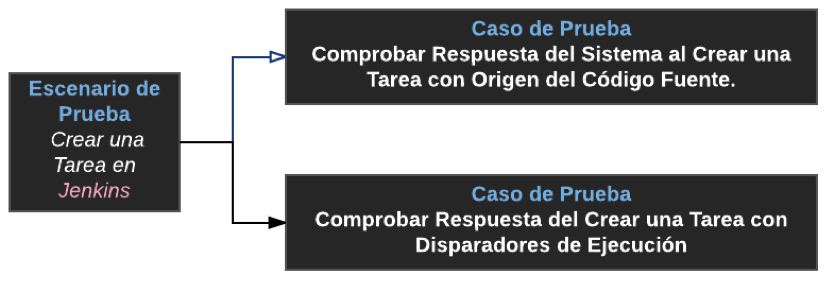
\includegraphics[width=0.55\linewidth]{img/p08.png}
	\caption{Diagrama de entrada y salida}
	\label{fig:MarcoTeorico}
\end{figure}

\begin{table}[H]
	\centering
	\begin{tabular}{  >{\centering\arraybackslash}m{0.5cm} >{\centering\arraybackslash}m{3cm}  >{\arraybackslash}m{4cm}  >{\arraybackslash}m{4cm}  >{\centering\arraybackslash}m{4cm} }
		\hline
		ID & Escenario & Caso de prueba & Entrada & Salida esperada\\
		\hline \hline
		06.1 & Crear una tarea en jenkins & Comprobar la respuesta del sistema al crear una tarea con origen de código Fuente & git@RepoCentral.uvici:root/php-proyecto-ci.git & Tarea creada\\
		06.1 & Crear una tarea en jenkins & Comprobar la Respuesta del sistema al crear una Tarea con disparadores de ejecución & CheckBox: Git push & Tarea creada\\
		\hline
	\end{tabular}
	\caption{Resumen de resultados}
	\label{tabla:autores}
\end{table}


\subsubsection{Prueba funcional 08}

\begin{figure}[H]
	\centering
	\includegraphics[width=0.55\linewidth]{img/p09.png}
	\caption{Diagrama de entrada y salida}
	\label{fig:MarcoTeorico}
\end{figure}

\begin{table}[H]
	\centering
	\begin{tabular}{  >{\centering\arraybackslash}m{0.5cm} >{\centering\arraybackslash}m{3cm}  >{\arraybackslash}m{4cm}  >{\arraybackslash}m{4cm}  >{\centering\arraybackslash}m{4cm} }
		\hline
		ID & Escenario & Caso de prueba & Entrada & Salida esperada\\
		\hline \hline
		06.1 & Integrar código fuente asociado a una tarea & Comprobar la respuesta del sistema al generar una construcción & push origin master  & Los archivos asociados al proyecto son recibidos correctamente.\\
		\hline
	\end{tabular}
	\caption{Resumen de resultados}
	\label{tabla:autores}
\end{table}

\subsection{Análisis de resultados}

En la ejecución de las pruebas Funcionales realizadas en la sección 10.1, se obtuvieron los siguientes resultados:

\begin{itemize}
	\item Casos de prueba ejecutados 22.
	\item Casos de prueba aprobados 22.
\end{itemize}

\section{Pruebas de sistema}

Debido a que la evaluación se aplica sobre la implementacion completa de la solución, pueden ser utilizadas distintos tipos de pruebas para examinar propiedades no funcionales del sistema.
La cantidad de usuarios que se espera soporte la infraestructura es proporcional a los recursos que poseen las maquinas que ejecutan las herramientas o componentes de Software. 
La actual distrubución de los recursos asegura un flujo, sin problemas, de a lo mas 100 usuarios concurrentes.

\begin{itemize}
	\item Pruebas de stress: Prueba conducida para evaluar un sistema o componente en sus limites de desempeño especificados o requeridos.
	\item Pruebas de carga: Pruebas realizadas para evaluar el cumplimiento de un sistema o un componente según los requisitos de rendimiento especificados.
\end{itemize}

\subsubsection{Plan de Pruebas - Repositorio Central}

\begin{figure}[H]
	\centering
	\includegraphics[width=0.28\linewidth]{img/plan1.png}
	\caption{Detalle del plan de pruebas}
	\label{fig:MarcoTeorico}
\end{figure}

\subsubsection{Plan de Pruebas - Servidor I.C}

\begin{figure}[H]
	\centering
	\includegraphics[width=0.28\linewidth]{img/plan2.png}
	\caption{Detalle del plan de pruebas}
	\label{fig:MarcoTeorico}
\end{figure}


\subsection{Pruebas de carga}

El plan de pruebas simula un hilo de Usuarios del tipo 'Alumno' que ejecuta una serie de peticiones. Haciendo uso de un receptor se interpreta la información del muestreador.

\subsubsection{Pruebas de Carga - Jenkins }

Para esta prueba se simula una carga de 100 usuarios/segundo en un periodo de 10 segundos.

\begin{figure}[H]
	\centering
	\includegraphics[width=0.5\linewidth]{img/p1.png}
	\caption{Diagrama de pruebas}
	\label{fig:MarcoTeorico}
\end{figure}

El gráfico de resultados muestra el throghput (color verde) del sistema y carga de datos en función del tiempo. El servidor logra resolver el 100 por ciento de las peticiones.

\begin{figure}[H]
	\centering
	\includegraphics[width=0.5\linewidth]{img/jmeter1.png}
	\caption{Grafico de resultados}
	\label{fig:MarcoTeorico}
\end{figure}

\subsubsection{Prueba de Carga - Gitlab}

Para esta prueba se simula una carga de 100 usuarios/segundo en un periodo de 10 segundos.

\begin{figure}[H]
	\centering
	\includegraphics[width=0.5\linewidth]{img/p3.png}
	\caption{Diagrama de pruebas}
	\label{fig:MarcoTeorico}
\end{figure}

El gráfico de resultados muestra el throghput del sistema y carga de datos en función del tiempo.

\begin{figure}[H]
	\centering
	\includegraphics[width=0.5\linewidth]{img/jmeter3.png}
	\caption{Grafico de resultados}
	\label{fig:MarcoTeorico}
\end{figure}

\subsubsection{Prueba de Carga - Gitlab}

Para esta prueba se simula una carga de 100 usuarios/segundos en periodos de 1 segundo. El servidor logra resolver el 100 por ciento de las peticiones.


\begin{figure}[H]
	\centering
	\includegraphics[width=0.15\linewidth]{img/p5.png}
	\caption{Diagrama de pruebas}
	\label{fig:MarcoTeorico}
\end{figure}

El gráfico de resultados muestra el throghput del sistema y carga de datos en función del tiempo. El servidor logra resolver el 100 por ciento de las peticiones.


\begin{figure}[H]
	\centering
	\includegraphics[width=0.25\linewidth]{img/jmeter5.png}
	\caption{Grafico de resultados}
	\label{fig:MarcoTeorico}
\end{figure}

\subsection{Pruebas de estrés}

\subsubsection{Prueba de Estrés - Jenkins}

Para esta prueba se simula una carga de 200 usuarios/segundos en periodos de 10 segundos.

\begin{figure}[H]
	\centering
	\includegraphics[width=0.5\linewidth]{img/p2.png}
	\caption{Diagrama de pruebas}
	\label{fig:MarcoTeorico}
\end{figure}

El sistema no resiste la prueba, el 80 por ciento de las peticiones llega al timeout.
En la Figura podemos apreciar un desempeño discontinuo.

\begin{figure}[H]
	\centering
	\includegraphics[width=0.5\linewidth]{img/jmeter2.png}
	\caption{Grafico de resultados}
	\label{fig:MarcoTeorico}
\end{figure}

\subsubsection{Prueba de Estrés - Gitlab}

Para esta prueba se simula una carga de 200 usuarios en un segundo.

\begin{figure}[H]
	\centering
	\includegraphics[width=0.3\linewidth]{img/p4.png}
	\caption{Diagrama de pruebas}
	\label{fig:MarcoTeorico}
\end{figure}

El gráfico de resultados muestra el throghput del sistema y carga de datos en función del tiempo. El servidor logra resolver el 100 por ciento de las peticiones.


\begin{figure}[H]
	\centering
	\includegraphics[width=0.4\linewidth]{img/jmeter4.png}
	\caption{Grafico de resultados}
	\label{fig:MarcoTeorico}
\end{figure}

\subsection{Análisis de resultados}

En la ejecución de las pruebas funcionales realizadas en la sección 10.2, se obtuvieron los siguientes resultados:

\begin{itemize}
	\item Casos de prueba ejecutados 5.
	\item Casos de prueba aprobados 5.
\end{itemize}



\section{Pruebas de validación}

Para esta prueba se considera un grupo de 3 alumnos, cada uno con una tarea especifica en la actividad.

\begin{figure}[H]
	\centering
	\includegraphics[width=0.5\linewidth]{img/validacion.png}
	\caption{Diagrama de validación}
	\label{fig:MarcoTeorico}
\end{figure}

\subsection{Análisis de resultados}
\begin{itemize}
	\item Casos de prueba ejecutados 1.
	\item Casos de prueba aprobados 1.
\end{itemize}

A partir de los datos obtenidos se puede afirmar que el sistema se comporta de forma correcta y constante. Las mediciones de CPU y memoria de la Figura 10.23 demuestra que el sistema soporta, en condiciones normales y limites, las operaciones especificadas.

\begin{figure}[H]
	\centering
	\includegraphics[width=0.4\linewidth]{img/validacion2.png}
	\caption{Desempeño del repositorio central}
	\label{fig:MarcoTeorico}
\end{figure}


\chapter{Implantación}

A continuación se describe el proceso de implantación que se llevó a cabo en el entorno real donde funciona el sistema, cada host conectados a la infraestructura puede enviar y recibir datos del repositorio central. 
Para mayor detalle sobre la instalación de cada una de las herramientas y tecnologías presentes en esta implantación leer el manual de implantación [Apendice A].

\section{Características del ambiente}

La escuela de Ingeniería Civil Informática de la Universidad de Valparaíso permite el uso de un servidor con las siguientes características.

\begin{itemize}
	
	\item Procesador: Intel(R) Xeon(R) CPU E5504, 2GHz. 
	\item Memoria Ram: 4GB
	\item Disco Duro: 320GB
	\item DVD: DV-28E-V
\end{itemize}


\section{Actividades previas a la implantación}

Instalación del sistema operativo Proxmox Virtual Environment 3.4 siguendo los pasos que se muestran a continuación:

\begin{itemize}
	\item Insertar el disco de instalación de Proxmox VE 3.4
	\item Particionar el disco duro que contendra el sistema operativo usando zfe 0.
	\item Configurar la red del servidor con la dirección IP: [10.100.6.4] Gw: [10.100.6.254] DNS: [10.50.1.16].
	\item Acceder al servicio web usando https://10.100.6.4:8006
\end{itemize}

\subsubsection{Contenedores OpenVZ}

Desde la interfaz grafica de Proxmox Virtual Environment 3.4 se crearón, iniciarón y actualizaron los siguientes servidores virtuales.

\begin{itemize}
	\item Contenedor OpenVZ: Repositorio Central
	\item Contenedor OpenVZ: Integración PHP
	\item Contenedor OpenVZ: Integración Java
	\item Contenedor OpenVZ: Servidor C
	\item Contenedor OpenVZ: Producción PHP
	\item Contenedor OpenVZ: Producción Java
\end{itemize}

\section{Actividades propias de la implantación}

La implantación del sistema se realizo siguiendo la secuencia de actividades descritas a continuación:

\begin{itemize}
	
	\item Primero se debe instalar el JDK development evironmet 1.8 y la herramienta Gitlab 8.10 en el Repositorio Central, para comprobar el funcionamiento, acceder a Gitlab desde un navegador con la siguiente dirección http://10.100.6.221
	\item Llevar a cabo la instalación de la herramienta Jenkins, PHP 5.6, composer y JDK 1.8 en el servidor de integración continua PHP, para comprobar su funcionamiento acceder a Jenkins desde un navegador con la siguiente dirección http://10.100.6.226:8080
	\item Llevar a cabo la instalación de la herramienta Jenkins y JDK 1.8 en el servidor de integración continua para el lenguaje PHP, para comprobar su funcionamiento acceder a Jenkins desde un navegador con la siguiente dirección http://10.100.6.227:8080. 
	\item En el Servidor C se instalo la herramienta gcc 1.7 y el editor de texto Vim.
	\item Instalación de PHP 5.6 y apache 2 en el servidor de despliegue PHP.
	\item Instalación de JDK 1.8 en el servidor de despliegue Java.
\end{itemize} 

\chapter{Conclusión}

Como resultado del trabajo realizado con respecto al desarrollo de la infraestructura, se pudo determinar que las herramientas y tecnologías permitieron el desarrollo y cumplimiento de requerimientos de este trabajo de título. Además, el uso conjunto de estas tecnologías ofrece una alternativa al proceso de desarrollo de software a la hora de ejecuctar actividades asociadas al ciclo de vida del software. Facilitando el trabajo entre los miembros de un equipo, que constantemente realiza cambios y pruebas a uno o varios proyectos.
Por otro lado esta solución integra herramientas y métodos de desarrollo que agilizan el proceso de desarrollo de software, asegurando experiencias mas realistas, traducibles en profesionales mas preparados, competentes y seguros.
\appendix
\chapter{Manual de implantación}\label{aped.A}

A continuación se especifican los detalles correspondientes a la instalación de tecnologías y herramientas del sistema.

\section{Instalar Proxmox VE 3.4}

\begin{itemize}
	\item Paso 1: Isertar la imagen de Proxmox en la unidad de DVD del servidor
	\item Paso 2: Seleccionar idioma y teclado, tal como se indica en la [Figura A.1].
	\begin{figure}[H]
		\centering
		\includegraphics[width=0.4\linewidth]{img/idioma.png}
		\caption{Selector de lenguaje}
		\label{fig:MarcoTeorico}
	\end{figure}
		\newpage
	\item Paso 3: Formatear disco usando ext 3 [Figura A.2].
	
	\begin{figure}[H]
		\centering
		\includegraphics[width=0.3\linewidth]{img/disco.png}
		\caption{Formatear disco duro}
		\label{fig:MarcoTeorico}
	\end{figure}

	\item Paso 4: Configurar los parametros de conección, tal como se indica [Figura A.3].
	
	\begin{figure}[H]
		\centering
		\includegraphics[width=0.4\linewidth]{img/red.png}
		\caption{Configurar red}
		\label{fig:MarcoTeorico}
	\end{figure}
	
\end{itemize}

\section{Instalar JDK Development Evironmet 1.8}

\begin{itemize}
	\item Agregar el respositorio webupd8team Java PPA, usando: add-apt-repository ppa:webupd8team/java
	\item Actualizar la source list con: apt-get update
	\item Instalar: apt-get install oracle-java8-installer
\end{itemize}

\subsection{Instalar PHP 5.6}

\begin{itemize}
	\item Agregar los repositorios a la source list usando: add-apt-repository ppa:ondrej/php5-5.6
	\item Actualizar: apt-get update
	\item Instalar: sudo apt-get install php5
\end{itemize}

\subsection{Instalar Gitlab 8.10}

\begin{itemize}
	
	\item Instalar y configurar las dependencias necesarias, usando: sudo apt-get install curl openssh-server ca-certificates postfix
	\item Agregar los packetes de gitlab 8.10 al servidor:  curl -sS https://packages.gitlab.com/install/repositories/gitlab/gitlab-ce/script.deb.sh | sudo bash
	\item instalar Gitlab: apt-get install gitlab-ce
	\item Configurar e inciar gitlab: gitlab-ctl reconfigure
\end{itemize}

\section{Instalar Jenkins}

\begin{itemize}
	\item Agregar repositorios a la sourcelist:sh -c echo deb http://pkg.jenkins.io/debianstable binary/  /etc/apt/sources.list.d/jenkins.list
	\item Acualizar: apt-get update
	\item instalar: apt-get install jenkins.
\end{itemize}


\section{Administrador Proxmox}

Este tipo de usuario puede acceder a la web GUI de Proxmox que facilita la creación, modificación y eliminación de contenedores \cite{proxmox}. Ingresar con la credencial que se muestra a continuación.

\begin{itemize}
	\item URL: https://10.100.6.4:8006
	\item Usuario: root
	\item Password: proxuvici
\end{itemize}

\section{Administrador Jenkins}

Este usuario puede crear tareas de integración \cite{jenkins} en la herramienta Jenkins para consumir datos del repositorio central. Ingresar con la credencial que se muestra a continuación.

\begin{itemize}
	\item URL: https://10.100.6.226:8080 [PHP]
	\item Usuario: root
	\item Password: gitlabuvici
\end{itemize}

\begin{itemize}
	\item URL: https://10.100.6.227:8080 [Java]
	\item Usuario: root
	\item Password: gitlabuvici
\end{itemize}

\section{Desarrollador Gitlab}

Para el uso de la herramienta Gitlab no hay restricciones de tipo de usuario, solo es requerido el registro de una cuenta para hacer uso de la herramienta \cite{gitlab}, acceder desde:

\begin{itemize}
	\item URL: http://10.100.6.221:80
\end{itemize}

\section{Flujo de trabajo}

El uso del sistema es como se muestra en la Figura B.1, en el contexto de la utilización de la metodología ágil [Feature Driven Development], se tendría el siguiente flujo de trabajo.

Primero un grupo de usuarios, trabaja en el desarrollo de una característica, con tiempo de implementación menor a dos días, estos desarrolladores hacen push (envían cambios al repositorio central) de sus últimas versiones. 
Luego el servidor de integración continua, Java o PHP, automáticamente ejecuta los test a las clases y construye una Build de la ultima versión del Master branch, esto a través de la configuración de un trigger, si todas las pruebas son exitosas, el servidor de integración continua se encarga de mover los archivos a los ambientes de producción correspondiente.

\begin{figure}[H]
	\centering
	\includegraphics[width=0.45\linewidth]{img/flujo.png}
	\caption{Flujo general del sistema}
	\label{fig:MarcoTeorico}
\end{figure}
